% Options for packages loaded elsewhere
\PassOptionsToPackage{unicode}{hyperref}
\PassOptionsToPackage{hyphens}{url}
\PassOptionsToPackage{dvipsnames,svgnames,x11names}{xcolor}
%
\documentclass[
  letterpaper,
  DIV=11,
  numbers=noendperiod]{scrreport}

\usepackage{amsmath,amssymb}
\usepackage{iftex}
\ifPDFTeX
  \usepackage[T1]{fontenc}
  \usepackage[utf8]{inputenc}
  \usepackage{textcomp} % provide euro and other symbols
\else % if luatex or xetex
  \usepackage{unicode-math}
  \defaultfontfeatures{Scale=MatchLowercase}
  \defaultfontfeatures[\rmfamily]{Ligatures=TeX,Scale=1}
\fi
\usepackage{lmodern}
\ifPDFTeX\else  
    % xetex/luatex font selection
\fi
% Use upquote if available, for straight quotes in verbatim environments
\IfFileExists{upquote.sty}{\usepackage{upquote}}{}
\IfFileExists{microtype.sty}{% use microtype if available
  \usepackage[]{microtype}
  \UseMicrotypeSet[protrusion]{basicmath} % disable protrusion for tt fonts
}{}
\makeatletter
\@ifundefined{KOMAClassName}{% if non-KOMA class
  \IfFileExists{parskip.sty}{%
    \usepackage{parskip}
  }{% else
    \setlength{\parindent}{0pt}
    \setlength{\parskip}{6pt plus 2pt minus 1pt}}
}{% if KOMA class
  \KOMAoptions{parskip=half}}
\makeatother
\usepackage{xcolor}
\usepackage{soul}
\setlength{\emergencystretch}{3em} % prevent overfull lines
\setcounter{secnumdepth}{5}
% Make \paragraph and \subparagraph free-standing
\ifx\paragraph\undefined\else
  \let\oldparagraph\paragraph
  \renewcommand{\paragraph}[1]{\oldparagraph{#1}\mbox{}}
\fi
\ifx\subparagraph\undefined\else
  \let\oldsubparagraph\subparagraph
  \renewcommand{\subparagraph}[1]{\oldsubparagraph{#1}\mbox{}}
\fi


\providecommand{\tightlist}{%
  \setlength{\itemsep}{0pt}\setlength{\parskip}{0pt}}\usepackage{longtable,booktabs,array}
\usepackage{calc} % for calculating minipage widths
% Correct order of tables after \paragraph or \subparagraph
\usepackage{etoolbox}
\makeatletter
\patchcmd\longtable{\par}{\if@noskipsec\mbox{}\fi\par}{}{}
\makeatother
% Allow footnotes in longtable head/foot
\IfFileExists{footnotehyper.sty}{\usepackage{footnotehyper}}{\usepackage{footnote}}
\makesavenoteenv{longtable}
\usepackage{graphicx}
\makeatletter
\def\maxwidth{\ifdim\Gin@nat@width>\linewidth\linewidth\else\Gin@nat@width\fi}
\def\maxheight{\ifdim\Gin@nat@height>\textheight\textheight\else\Gin@nat@height\fi}
\makeatother
% Scale images if necessary, so that they will not overflow the page
% margins by default, and it is still possible to overwrite the defaults
% using explicit options in \includegraphics[width, height, ...]{}
\setkeys{Gin}{width=\maxwidth,height=\maxheight,keepaspectratio}
% Set default figure placement to htbp
\makeatletter
\def\fps@figure{htbp}
\makeatother
\newlength{\cslhangindent}
\setlength{\cslhangindent}{1.5em}
\newlength{\csllabelwidth}
\setlength{\csllabelwidth}{3em}
\newlength{\cslentryspacingunit} % times entry-spacing
\setlength{\cslentryspacingunit}{\parskip}
\newenvironment{CSLReferences}[2] % #1 hanging-ident, #2 entry spacing
 {% don't indent paragraphs
  \setlength{\parindent}{0pt}
  % turn on hanging indent if param 1 is 1
  \ifodd #1
  \let\oldpar\par
  \def\par{\hangindent=\cslhangindent\oldpar}
  \fi
  % set entry spacing
  \setlength{\parskip}{#2\cslentryspacingunit}
 }%
 {}
\usepackage{calc}
\newcommand{\CSLBlock}[1]{#1\hfill\break}
\newcommand{\CSLLeftMargin}[1]{\parbox[t]{\csllabelwidth}{#1}}
\newcommand{\CSLRightInline}[1]{\parbox[t]{\linewidth - \csllabelwidth}{#1}\break}
\newcommand{\CSLIndent}[1]{\hspace{\cslhangindent}#1}

\usepackage{multirow}
\usepackage{array} 
\usepackage{hhline}
\usepackage{pgfplots}
\usepackage{multicol}
\KOMAoption{captions}{tableheading}
\makeatletter
\@ifpackageloaded{tcolorbox}{}{\usepackage[skins,breakable]{tcolorbox}}
\@ifpackageloaded{fontawesome5}{}{\usepackage{fontawesome5}}
\definecolor{quarto-callout-color}{HTML}{909090}
\definecolor{quarto-callout-note-color}{HTML}{0758E5}
\definecolor{quarto-callout-important-color}{HTML}{CC1914}
\definecolor{quarto-callout-warning-color}{HTML}{EB9113}
\definecolor{quarto-callout-tip-color}{HTML}{00A047}
\definecolor{quarto-callout-caution-color}{HTML}{FC5300}
\definecolor{quarto-callout-color-frame}{HTML}{acacac}
\definecolor{quarto-callout-note-color-frame}{HTML}{4582ec}
\definecolor{quarto-callout-important-color-frame}{HTML}{d9534f}
\definecolor{quarto-callout-warning-color-frame}{HTML}{f0ad4e}
\definecolor{quarto-callout-tip-color-frame}{HTML}{02b875}
\definecolor{quarto-callout-caution-color-frame}{HTML}{fd7e14}
\makeatother
\makeatletter
\makeatother
\makeatletter
\@ifpackageloaded{bookmark}{}{\usepackage{bookmark}}
\makeatother
\makeatletter
\@ifpackageloaded{caption}{}{\usepackage{caption}}
\AtBeginDocument{%
\ifdefined\contentsname
  \renewcommand*\contentsname{Table of contents}
\else
  \newcommand\contentsname{Table of contents}
\fi
\ifdefined\listfigurename
  \renewcommand*\listfigurename{List of Figures}
\else
  \newcommand\listfigurename{List of Figures}
\fi
\ifdefined\listtablename
  \renewcommand*\listtablename{List of Tables}
\else
  \newcommand\listtablename{List of Tables}
\fi
\ifdefined\figurename
  \renewcommand*\figurename{Figure}
\else
  \newcommand\figurename{Figure}
\fi
\ifdefined\tablename
  \renewcommand*\tablename{Table}
\else
  \newcommand\tablename{Table}
\fi
}
\@ifpackageloaded{float}{}{\usepackage{float}}
\floatstyle{ruled}
\@ifundefined{c@chapter}{\newfloat{codelisting}{h}{lop}}{\newfloat{codelisting}{h}{lop}[chapter]}
\floatname{codelisting}{Listing}
\newcommand*\listoflistings{\listof{codelisting}{List of Listings}}
\makeatother
\makeatletter
\@ifpackageloaded{caption}{}{\usepackage{caption}}
\@ifpackageloaded{subcaption}{}{\usepackage{subcaption}}
\makeatother
\makeatletter
\@ifpackageloaded{tcolorbox}{}{\usepackage[skins,breakable]{tcolorbox}}
\makeatother
\makeatletter
\@ifundefined{shadecolor}{\definecolor{shadecolor}{rgb}{.97, .97, .97}}
\makeatother
\makeatletter
\makeatother
\makeatletter
\makeatother
\ifLuaTeX
  \usepackage{selnolig}  % disable illegal ligatures
\fi
\IfFileExists{bookmark.sty}{\usepackage{bookmark}}{\usepackage{hyperref}}
\IfFileExists{xurl.sty}{\usepackage{xurl}}{} % add URL line breaks if available
\urlstyle{same} % disable monospaced font for URLs
\hypersetup{
  pdftitle={Fundamentos de Economía},
  pdfauthor={Sebastián Cea, Joaquín Fernández, Reimundo Fuenzalida},
  colorlinks=true,
  linkcolor={blue},
  filecolor={Maroon},
  citecolor={Blue},
  urlcolor={Blue},
  pdfcreator={LaTeX via pandoc}}

\title{Fundamentos de Economía}
\author{Sebastián Cea, Joaquín Fernández, Reimundo Fuenzalida}
\date{Invalid Date}

\begin{document}
\maketitle
\ifdefined\Shaded\renewenvironment{Shaded}{\begin{tcolorbox}[borderline west={3pt}{0pt}{shadecolor}, boxrule=0pt, enhanced, interior hidden, breakable, frame hidden, sharp corners]}{\end{tcolorbox}}\fi

\renewcommand*\contentsname{Table of contents}
{
\hypersetup{linkcolor=}
\setcounter{tocdepth}{2}
\tableofcontents
}
\bookmarksetup{startatroot}

\hypertarget{prefacio}{%
\chapter*{Prefacio}\label{prefacio}}
\addcontentsline{toc}{chapter}{Prefacio}

\markboth{Prefacio}{Prefacio}

~ Este apunte nace de las notas tomadas por Reimundo Fuenzalida el
primer semestre del 2022. A través de los semestres sucesivos ha ido
integrando revisiones, ejercicios y las ayudantías que se han hecho a
través de los años.

\bookmarksetup{startatroot}

\hypertarget{introducciuxf3n-a-la-economuxeda.}{%
\chapter{Introducción a la
economía.}\label{introducciuxf3n-a-la-economuxeda.}}

\hypertarget{definiciuxf3n-y-clasificaciuxf3n-de-la-economuxeda}{%
\section{Definición y clasificación de la
economía:}\label{definiciuxf3n-y-clasificaciuxf3n-de-la-economuxeda}}

~ La palabra economía significa literalmente ``administración del
hogar'',\footnote{Del griego \emph{oikos} y \emph{nomos}.} pero su
definición es ``el estudio del modo en que la sociedad asigna recursos
escasos a necesidades múltiples''. Los recursos pueden ser o no escasos,
para los que lo son se le llaman recursos económicos, y para los que no
recursos libres. Los libres no tienen un valor económico, por lo tanto,
tampoco tienen dueños. A ambos bienes las personas les otorgan un
valor.\footnote{Se puede distinguir entre valor de uso y valor de intercambio de acuerdo a David Ricardo.}
En particular, los recursos escasos generan un \emph{trade-off}, por lo
que surge un problema para asignar su valor.

~ \{\color{red}La economía estudia el modo en que la sociedad gestiona
sus recursos escasos, es más, el problema fundamental de la economía es
la \textbf{escasez de recursos.} Si no existiera este problema, la
ciencia de la economía no existiría. Esta ciencia busca entender el modo
en que se interrelacionan las personas a nivel económico, es decir, en
el mercado. Para que exista este último termino, tiene que haber
compradores y vendedores que realicen transacciones de entre ellos, ya
sea de forma física o no.\}

\color{black}

~ Existen dos tipos de niveles de estudio de la economía, la
microeconomía que estudia unidades económicas individuales y la
macroeconomía que estudia variables económicas agregadas. Un sistema
económico es la forma en que se asignan los recursos, existen los
centralizados, es decir, los que un solo planificador asigna los
recursos, los descentralizados, que la sociedad en general asigna los
recursos y los mixtos, que asignan algunos bienes el estado y el otro la
sociedad. La econometría es el estudio de estas cuestiones basado en
técnicas estadísticas para testear postulados macroeconómicos y
microeconómicos.

\underline{\textbf{En resumen:}}

\begin{table}[htb]
    \centering
    \begin{tabular}{|p{20mm}|p{30mm}|p{45mm}|p{45mm}|}
        \hline
        Tipo & Clasificación & Definición & Ejemplo \\ \hline
        \multirow{3}{3cm}{Sistema Económico:} & Centralizado & \hspace{2mm} Un solo agente administra todos los bienes. & \hspace{2mm} El gobierno regulariza, produce y administra todos los bienes.\\ \cline{2-4}
        & Descentralizado & \hspace{2mm} Los bienes son repartidos por la sociedad. Rol ejercido por el mercado. & \hspace{2mm} Varias empresas producen un mismo bien, por lo que la sociedad escoge a quien comprar.\\ \cline{2-4}
        & Mixto & \hspace{2mm} Algunos bienes o mercados son centralizados y otros descentralizados. & \hspace{2mm} El petróleo tiene intervenidos los precios y el gobierno tiene el monopolio de distribución. En contraste, el maíz es producido por distintos semilleros.\\ \cline{1-4}
        \multirow{3}{3cm}{Niveles de Estudio:} & Microeconomía & \hspace{2mm} Estudio de unidades económicas individuales. & \hspace{2mm} La administración de una familia o empresa. \\ \cline{2-4}
        & Macroeconomía & \hspace{2mm} Estudio de unidades económicas agregadas. & \hspace{2mm} La administración de un país en base a variables como el PIB, la UF, el desempleo, etc. \\ \cline{1-4}
        \multirow{3}{3cm}{Recursos:} & Económicos & \hspace{2mm} Tienen valor económico y son escasos. & \hspace{2mm} El trigo, Los bienes raíces o el agua. \\ \cline{2-4}
        & Libres & \hspace{2mm} No tienen valor económico. & \hspace{2mm} El sol. \\ \cline{1-4}
    \end{tabular}
    \caption{Clasificación de la economía.}
    \label{tabla:final}
\end{table}

\hypertarget{los-diez-principios-de-la-economuxeda}{%
\section{Los Diez Principios de la
economía:}\label{los-diez-principios-de-la-economuxeda}}

~ Los diez principios de la economía son afirmaciones que muestran
hechos relevantes del análisis económico de acuerdo a
\cite{mankiw_principios_2012}. Estos responden a tres preguntas.

\begin{enumerate}
\def\labelenumi{\arabic{enumi}.}
\tightlist
\item
  ¿Cómo los individuos toman decisiones? (eficiencia, escasez, costos de
  oportunidad e incentivos.)
\item
  ¿Cómo interactúan los individuos? (derechos de propiedad, fallas del
  mercado y externalidades.)
\item
  ¿Cómo funciona la economía en su conjunto? (productividad, inflación y
  ciclo económico)
\end{enumerate}

~ En la siguiente tabla se explican estas proposiciones:

\begin{table}[H]
    \centering
    \scalebox{0.95}{\begin{tabular}{|p{20mm}|p{30mm}|p{37mm}|p{53mm}|}
        \hline
        Numero: & Principio: & Explicación: & Ejemplo: \\ \hline
        1 & \hspace{2mm} “Los individuos enfrentan disyuntivas.” & \hspace{2mm} Esto se refiere a escoger una cosa u otra. & \hspace{2mm} Los dos tipos de disyuntivas son: \par \hspace{2mm} \underline{Eficiencia}, es decir como la sociedad aprovecha al máximo sus recursos. \par \hspace{2mm} \underline{Equidad}, como la sociedad distribuye equitativamente los recursos. \par \hspace{2mm} Ambos tipos de disyuntiva son dependientes uno al otro. \\ \hline
        2 & \hspace{2mm} “El costo de algo es aquello a lo que se renuncia por obtenerlo.” & \hspace{2mm} Esto se refiere a \underline{“el costo} \underline{oportunidad”}, o bien, a lo que se renuncia por obtener otro bien. También se le conoce como \textit{precio sombra}. & \hspace{2mm} Comprar para el desayuno un plátano renunciando a comer una manzana. \\ \hline
        3 & \hspace{2mm} “Pensamiento marginal.” & \hspace{2mm} Solo venderemos algo si la \textit{ganancia marginal} supera el \textit{costo marginal}. & \hspace{2mm}  El costo de producir manzanas, con todos los gastos que conlleva, es menor al beneficio y por lo tanto al ingreso que me proporciona este. \\ \hline
        4 & \hspace{2mm} “Los individuos responden a incentivos.” & \hspace{2mm} Cuando hay cambios en los costos, beneficios o se hace propaganda, o publicidad en un producto. & \hspace{2mm} Si el plátano vale más que la naranja, compraré naranja, pero si el plátano hace mejor para la salud, compraré plátano. \\ \hline
        5 & \hspace{2mm} “El comercio puede mejorar el bienestar de todos.” & \hspace{2mm} Cuando hay \underline{competencia} todos ganan, o al menos, no se pierde. Hay más especialización y se intenta abaratar los costos sin perder la especialización. & \hspace{2mm} Chile puede producir autos, pero no será eficiente, porque china lo hace mejor, pero si puede vender cerezas, ya que, chile es superior a china en ese rubro. \\ \hline
        \end{tabular}}
    \caption{Principios de la economía (1-5).}
    \label{tabla:final}
\end{table}

\begin{table}[H]
    \centering
    \begin{tabular}{|p{16mm}|p{30mm}|p{59mm}|p{40mm}|}
        \hline
        Numero: & Principio: & Explicación: & Ejemplo: \\ \hline
        6 & \hspace{2mm} “Normalmente, los mercados son un buen mecanismo de asignación de recursos.” & \hspace{2mm} Primer teorema del bienestar social \underline{(PTB):} La mano invisible de Adam Smith dice que los mercados se regulan solos y lo hacen bien. {\color{red}{Este principio concluye que es el egoísmo individual, con relación a la economía, el que trae mayores beneficios a la sociedad y no la solidaridad de los individuos.}}    & \hspace{2mm} Las personas producirán y comprarán pan según el precio que tengan las panaderías y la calidad que tenga. \\ \hline
        7 & \hspace{2mm} “En ocasiones, el gobierno puede mejorar los resultados del mercado.” & \hspace{2mm} Segundo teorema del bienestar social \underline{(STB):} Por fallas del mercado, externalidades o poder de mercado. & \hspace{2mm} Impuesto a las empresas que contaminan, evitan una externalidad negativa ayudando al común de la gente. \\ \hline
        8 & \hspace{2mm} “El nivel de vida de un país depende de su capacidad para producir bienes y servicios.” & \hspace{2mm} Un punto que afecta es el \underline{PIB per cápita}, lo que produce el país dividido su población. Y la \underline{productividad}, que es la cantidad de bienes y servicios producidos por cada unidad de trabajo. & \hspace{2mm} Chile no solo tiene un PIB per cápita mayor que el de sus vecinos de la región, sino que también tiene farmacias, supermercados, etc. \\ \hline
        9 & \hspace{2mm} “Los precios suben cuando el Banco Central imprime mucho dinero” & \hspace{2mm} \underline{Inflación:} o también desvalorización del valor de la moneda por su gran cantidad de circulación. & \hspace{2mm} Al imprimir más billetes hay más plata circulando, esto hace que se gaste más plata, pero que al mismo tiempo esta plata tenga menos valor, ya que, la cantidad de bienes y servicios en la economía siguen siendo los mismos. \\ \hline
        10 & \hspace{2mm} “La sociedad enfrenta una disyuntiva a corto plazo entre inflación y desempleo.” & \hspace{2mm} \underline{Curva de \cite{phillips_relation_1958}:} hay un intercambio de inflación por desempleo. \underline{Ciclo económico:} Hay una variación de intensidad en la actividad económica, como el empleo y la producción. & \hspace{2mm} La gran depresión (1929). \\ \hline
    \end{tabular}
    \caption{Principios de la economía (6-10).}
    \label{tabla:final}
\end{table}

\hypertarget{modelos-y-supuestos}{%
\section{Modelos y supuestos:}\label{modelos-y-supuestos}}

~ El análisis de un modelo económico toma en cuenta supuestos, los
modelos económicos analizan:

\begin{enumerate}
\def\labelenumi{\arabic{enumi}.}
\tightlist
\item
  Un problema y su información relevante.
\item
  deducciones lógicas con ayuda de las matemáticas.
\end{enumerate}

~ Y el supuesto de este modelo se centra en:

\begin{enumerate}
\def\labelenumi{\arabic{enumi}.}
\tightlist
\item
  cuales son estos.
\item
  ¿son algunos mejores que otros?, ¿son más necesarios?, ¿son
  suficientes?
\end{enumerate}

~ A base de estos conceptos se hace un análisis positivo y otro
negativo.

\begin{tcolorbox}[enhanced jigsaw, opacitybacktitle=0.6, toprule=.15mm, titlerule=0mm, colframe=quarto-callout-note-color-frame, toptitle=1mm, colback=white, bottomtitle=1mm, breakable, opacityback=0, coltitle=black, left=2mm, arc=.35mm, leftrule=.75mm, rightrule=.15mm, bottomrule=.15mm, title=\textcolor{quarto-callout-note-color}{\faInfo}\hspace{0.5em}{Ejemplo}, colbacktitle=quarto-callout-note-color!10!white]

~ ¿Cómo afectará un aumento de la inflación en el mercado de la comida
rápida?\footnotemark{}

~ En este caso solo tenemos un supuesto, que es el aumento de la
inflación y el problema a resolver es cómo influye esto en este mercado.
Dos posibles análisis de respuesta:

\begin{itemize}
\item
  Si el causante de la inflación es un aumento del salario mínimo: Los
  sueldos aumentan y la gente tendrá más dinero para gastar. Por
  consecuencia, el aumento del gasto de las personas va a generar
  escasez y esta escasez un aumento de los precios. Esos precios siendo
  los del mercado de comida rápida también.
\item
  Si hay una mayor emisión/impresión de papel moneda (billetes): La
  gente tiene más acceso a crédito y podrá gastar más dinero, lo que
  generará escasez y aumento de precios. En particular, también
  afectando los precios en el mercado de comida rápida.
\end{itemize}

\end{tcolorbox}

\footnotetext{Ver
\href{https://www.ine.gob.cl/estadisticas/economia/indices-de-precio-e-inflacion/indice-de-precios-al-consumidor}{Boletín
del Índice de Precios al Consumidor (IPC) en Chile}, que es la medida
con la que se monitorea la inflación}

\hypertarget{fronteras-de-posibilidades-de-producciuxf3n-o-fpp}{%
\section{Fronteras de posibilidades de producción o
FPP:}\label{fronteras-de-posibilidades-de-producciuxf3n-o-fpp}}

~ Hay tres términos que se relacionan cuando hablamos de posibilidades
de producción:

~ Tenemos los \ul{\textbf{los factores productivos}}, es decir, el uso
que se le da a el capital humano, los recursos naturales, el capital
físico y las tecnologías para producir el bien.

~ El \ul{\textbf{conjunto de posibilidades de producción}} es el grupo
que reúne los distintos resultados al decidir fabricar una combinación
de bienes con factores productivos variables que sirven como insumo en
todos los procesos productivos que se analizan. Así la
\ul{\textbf{frontera de posibilidades de producción (FPP)}} se
representa por las combinaciones de producción (en la frontera del
conjunto de posibilidades) que puede tener una economía teniendo en
cuenta que sus factores productivos se utilizan de forma eficiente (es
decir, no se puede producir más con otra asignación de recursos).

~ Finalmente tenemos el \ul{\textbf{costo de oportunidad}} que, en
simples palabras, es cuanto de un producto (por ejemplo \(y_1\) en la
Figure~\ref{fig-FPP} ) se pierde al aumentar la producción en una cierta
cantidad de otro bien (por ejemplo \(y_2\) en la Figure~\ref{fig-FPP}).

~ \textbf{\ul{FPP de forma matemática y gráfica:}}

~ Digamos que tenemos un factor o insumo productivo limitado \(\bar x\).
Si queremos crear una unidad del bien \(y_1\) se gastarán \(a_1\)
unidades del factor, y al fabricar una unidad del bien \(y_2\) se usaran
\(a_2\) unidades del factor. Si lo vemos matemáticamente tenemos una
suerte de restricción presupuestaria que nos obliga a explicar el uso de
recursos \(\bar x\) como una decisión de producción \((y_1,y_2)\):

\begin{equation}\protect\hypertarget{eq-FPP}{}{
\bar x=a_1y_1+a_2y_2
}\label{eq-FPP}\end{equation} ~ En consecuencia, la máxima cantidad de
\(y_n\) para \(n = 1\) ó \(2\), se representa como: \[
\bar x=a_ny_n \Leftrightarrow y_n=\frac{\bar x}{a_n}
\]

~ Entonces gráficamente podemos representar tanto la frontera (con la
ecuación Equation~\ref{eq-FPP}) como la región bajo la misma que
representa combinaciones de producción factibles que no maximizan la
cantidad producida (ineficientes):

\begin{figure}

{\centering \includegraphics[width=0.4\textwidth,height=\textheight]{intro_files/figure-pdf/fig-FPP-1.pdf}

}

\caption{\label{fig-FPP}FPP entre los bienes \(y_1\) e \(y_2\).}

\end{figure}

~ Note que el coeficiente \(a_i\) nos explica los requerimientos de
insumo por cantidad producida. De esta forma, podemos interpretar
\(a_i\cdot y_i\) como la demanda del insumo dependiente en la cantidad
que se quiere producir. Denotemos esa demanda por
\(x_i(y_i)=a_i\cdot y_i\). Si no hay otros insumos en el proceso de
producción, entonces al invertir \(x_i(y_i)\) obtendremos la función de
producción. En el caso anteriormente mencionado, sería
\(y_i(x_i)=\frac{x_i}{a_i}\). Con este ejemplo podemos ver que si
aumentamos marginalmente la contratación del insumo \(i\), entonces la
producción aumentará en un valor de \(\frac{1}{a_i}\). Ese valor,
equivalente a la derivada de la función de producción respecto del
factor productivo, es lo que se conoce como productividad marginal. En
conclusión, el inverso del coeficiente \(a_i\) es la productividad
marginal del insumo en el sector \(i\).

\begin{tcolorbox}[enhanced jigsaw, opacitybacktitle=0.6, toprule=.15mm, titlerule=0mm, colframe=quarto-callout-note-color-frame, toptitle=1mm, colback=white, bottomtitle=1mm, breakable, opacityback=0, coltitle=black, left=2mm, arc=.35mm, leftrule=.75mm, rightrule=.15mm, bottomrule=.15mm, title=\textcolor{quarto-callout-note-color}{\faInfo}\hspace{0.5em}{Ejemplo}, colbacktitle=quarto-callout-note-color!10!white]

~ Un granjero tiene \(216\) hectáreas, si planta lechuga podrá producir
\(1/3\) toneladas por hectárea. Si cosecho \(34\) toneladas de lechuga,
y el resto de las hectáreas las usó para sembrar maíz, sabemos que la
producción de maíz es igual a \(57\) toneladas. Grafique la FPP.

\textbf{Respuesta:}

~ \ul{Paso I: Interpretar.}

~ Diremos que \(y_1\) es la cantidad de lechuga e \(y_2\) la cantidad de
maíz, ambos se miden en toneladas, el costo de oportunidad para la
lechuga en base al maíz estará en función de \(a_1\) y \(a_2\). La
escasez estará dada por el factor limitante que es \(\bar h\) y fijo en
\(216\) de acuerdo al enunciado.

~ Si por hectárea se produce \(1/3\) de tonelada de lechuga, entonces
\(\frac{1}{a_1}=\frac{1}{3}\). Utilizando la ecuación
Equation~\ref{eq-FPP} para \(y_1=34\) e \(y_2=57\), es decir asumiendo
tecnologías con un solo insumo y lineales, tenemos lo siguiente si
reemplazamos la información previa:

\[\bar h=216=\underbrace{3}_{\frac{1}{a_1}=\frac{1}{3}}\cdot \underbrace{34}_{y_1}+a_2\cdot \underbrace{52}
_{y_2}.\]

~ \ul{Paso II: Escribir las ecuaciones y resolver.}

~ Entonces, es posible obtener \(a_2\) resolviendo lo anterior:

\[
\bar h=a_1y_1+a_2y_2
\] \[
216= 3y_1+a_2y_2 \Leftrightarrow 216=3 \cdot 34+57a_2
\] \[
216-102=34+57a_2 \Leftrightarrow \\frac{114}{57}=a_2
\] \[
a_2=2
\]

~ En resumen, del enunciado hemos interpretado cuánto vale \(a_1\).
Luego, hemos deducido cuánto vale \(a_2\) para poder completar la
ecuación de la FPP y así tener la información para graficarla. Así, la
ecuación resulta:

\[
\bar h = 3y_1+2y_2
\]

~ \ul{Paso III: Calcular cantidades máximas de cada bien.}

\[
216=3y_1 \Leftrightarrow y_1=72
\]

\[
216h=2y_2 \Leftrightarrow y_2=108
\]

~ \ul{Paso IV: Hacer el gráfico.}

\begin{figure}[H]

{\centering \includegraphics[width=0.6\textwidth,height=\textheight]{intro_files/figure-pdf/unnamed-chunk-2-1.pdf}

}

\end{figure}

\end{tcolorbox}

\hypertarget{especializaciuxf3n-y-comercio}{%
\section{Especialización y
comercio:}\label{especializaciuxf3n-y-comercio}}

~ Al comparar dos productores puede que cada uno use más unidades de
factor productivo para hacer un bien que otro. Entonces definiremos dos
conceptos:

~ \textbf{Ventaja absoluta:} es la habilidad por producir el mismo bien,
pero con menos unidades de factor.

~ \textbf{Ventaja comparativa:} Habilidad de un productor para producir
un mismo bien con menos costo de oportunidad.

~ ¿Como se calcula cada uno?

~ Tenemos dos productores estos son el productor ``D'' y el productor
``E'', también dos bienes que requieren de los mismos factores de
producción uno es el bien ``b'', que cuesta producirlo \(a_1\) en D y
\(a_2\) en E, y el otro es el bien ``c'', que cuesta producirlo \(a_3\)
en D y \(a_4\) en E. Además el factor productivo limitante los
denotaremos como x.

~ La ecuación para comparar la producción de sus bienes es la siguiente:

\[
\begin{matrix}
D: x = a_1 b + a_2 c\\
E: x = a_3 b + a_4 c\\
\end{matrix}
\]

~ \ul{Ejercicio resuelto:}

~ En la chocolatería E se hace chocolate dulce ``d'' y le cuesta
producirlo 10 gramos de cacao, pero en la chocolatería B le cuesta
producirlo 15 gramos de cacao. Ambos producen también chocolate amargo
``a'', a la chocolatería E le cuesta 12 gramos de cacao producirlo,
mientras que en la B le cuesta 20 gramos.

~ Si los dos tienen la misma cantidad de caco ``x'' ¿Quién tiene la
ventaja absoluta en los distintos bienes? Y ¿Quién tiene la ventaja
comparativa en estos chocolates?

\textbf{Respuesta:}

~ \ul{Paso I: Escribir la ecuación.}

\[
\begin{matrix}    E: $x = 10d + 12a$ \\    B: $x = 15d + 20a$\end{matrix}
\]

~ \ul{Paso II: Calcular la ventaja absoluta.}

~ Para esto, solo tenemos que comparar los coeficientes de cada bien con
el de la otra chocolatería, el de menos coeficiente, es el que tiene
mayor ventaja absoluta:

\[
\begin{matrix}    \text{d: $E = 10$, $B = 15$} \\    \text{E tiene la ventaja absoluta.}\\    \text{a: $E = 12$, $B = 20$} \\    \text{E tiene la ventaja absoluta.}\end{matrix}
\]

~ \ul{Paso III: Calcular la ventaja comparativa.}

~ hay que tener en cuenta que, al estar comparando ventajas
comparativas, no se usan signos negativos.

\begin{center}
        E : $10d = 12a$ \\
        B : $15d = 20a$
\end{center}

~ Luego:

\[
\textrm{E :} d = a\frac{12}{10}
\] \[
\textrm{B :} d = a\frac{20}{15}
\]

\[
\textrm{E :} a = d\frac{10}{12}
\] \[
\textrm{B :} a = d\frac{15}{20}
\] ~ Se compara, el que tenga menor coeficiente tiene la ventaja:

\begin{table}[H]
    \centering
    \begin{tabular}{|p{10mm}|p{10mm}|p{10mm}|p{25mm}|}
        \hline
        X & E: & B: & Tiene la ventaja comparativa: \\ \hline
        d = \par & $a\dfrac{18}{15}$ & $a\dfrac{20}{15}$ & E \\ \hline
        a = \par & $d\dfrac{10}{12}$ & $d\dfrac{9}{12}$ & B \\ \hline
    \end{tabular}
\end{table}

\bookmarksetup{startatroot}

\hypertarget{funcionamiento-de-los-mercados.}{%
\chapter{Funcionamiento de los
mercados.}\label{funcionamiento-de-los-mercados.}}

\hypertarget{costos-de-producciuxf3n}{%
\section{Costos de producción:}\label{costos-de-producciuxf3n}}

\[
\pi = IT-CT \Leftrightarrow \pi = IT-CT(H_1,H_2,L,K)
\]

~ Donde ``\(\pi\)'' es el beneficio, ``\(IT\)'' el ingreso, y ``\(CT\)''
es el gasto. Y donde ``\(H_1\)'' es materia prima, estos son los
materiales que se extraen directamente de la naturaleza, como la madera.
``\(H_2\)'' es insumos, a diferencia de la materia prima son elementos
ya procesados, como el cartón. ``\(L\)'' es mano de obra, es el gasto
que se hace por tener empleados, por ejemplo, el sueldo. y ``\(K\)''
gastos generales, son los gastos que se hacen constantemente, como el
arriendo de un lugar.

~ \ul{Ejercicio resuelto:}

~ Se tiene una ferretería que tiene de gastos \$100 en materia prima,
\$150 en insumos, \$50 en mano de obra y tiene de ingresos y beneficios
\$850 y \$350 respectivamente ¿Cuánto son sus gastos generales?

~ \ul{Respuesta:}

~ Se tiene una ferretería que tiene de gastos \$100 en materia prima,
\$150 en insumos, \$50 en mano de obra y tiene de ingresos y beneficios
\$850 y \$350 respectivamente ¿Cuánto son sus gastos generales?

~ \textbf{Respuesta:}

~ Reemplazamos en \(\pi = IT-CT(H_1,H_2,L,K)\). \[
350 = 850-(100+150+50+K)
\]

\[
350 = 850-300-K
\]

\[
350 = 550-K
\]

\[
K = 200
\]

\hypertarget{oferta}{%
\section{Oferta:}\label{oferta}}

~ La oferta, en breves palabras, es el mínimo valor al cual se está
dispuesto a vender determinada cantidad. Donde \(Q\) es la cantidad que
se va a producir, \(a\) es una contante y \(b>0\) es la pendiente si
asumimos una forma funcional lineal para la relación. Así la función
determina el valor del bien que se produce es:

\[
P(Q)=a+bQ
\]

~ Para entender bien mostraremos un gráfico, donde (utilizando punto
para los decimales) \(a=0.5\), \(b=0.5\):

\begin{multicols}{2}
\begin{table}[H]
    \centering
    \begin{tabular}{|p{25mm}|p{25mm}|}
        \multicolumn{2}{c}{Tabla de oferta:} \\ 
        \hline
        Precio ($P$) & Cantidad ($Q$) \\ \hline
        1 & 1 \\ \hline
        1,5 & 2 \\ \hline
        2 & 3 \\ \hline
        2,5 & 4 \\ \hline
        3 & 5 \\ \hline
        3,5 & 6 \\ \hline
        4 & 7 \\ \hline
        4,5 & 8 \\ \hline
        5 & 9 \\ \hline
        \end{tabular}
\end{table}


\begin{center}
    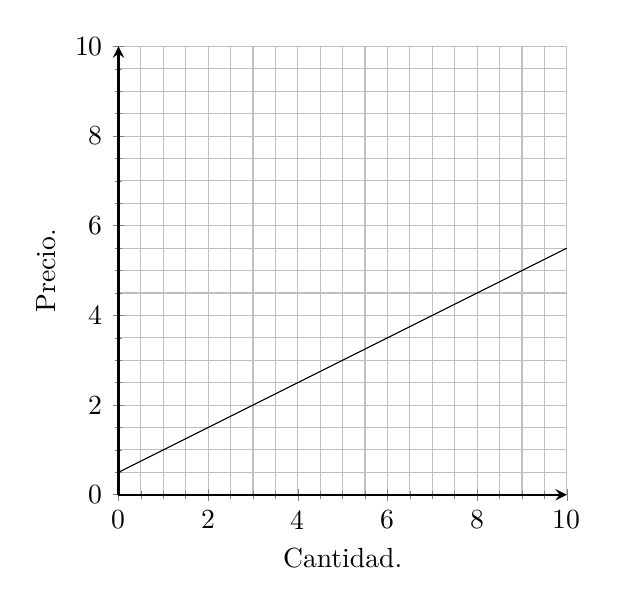
\begin{tikzpicture}
    \begin{axis}[grid=both,
    unit vector ratio*=1 1 1,
    axis x line=bottom,
    axis y line=left,
    axis line style=thick,
    xmax=10,xmin=0,
    ymax=10,ymin=0,
    xtick={0,2,4,6,8,10},
    ytick={0,2,4,6,8,10},
    minor tick num=3,
    xlabel=Cantidad.,
    ylabel=Precio.,
    ylabel near ticks,
    ylabel style={align=center},
    xlabel near ticks,
    ]
    
    \addplot[draw, smooth] coordinates {(0,0.5) (10,5.5)};
    \end{axis}
    \end{tikzpicture}
\end{center}
\end{multicols}

\hypertarget{demanda}{%
\section{Demanda:}\label{demanda}}

~ Mientras que la oferta se enfoca en el productor la demanda ve el
comportamiento de los consumidores. La cantidad demandada es cuanto está
dispuesto a comprar el consumidor para un determinado precio. La ley de
demanda dice que a mayor precio habrá una menor cantidad demandada.
Dicha relación, asumiendo una forma lineal se puede re-escribir como:

\[
P(Q)=a-bQ
\] ~ Para los valores \(a=21\), \(b=0.8\), que podría ser el mismo caso
anterior, el gráfico sería así:

\begin{multicols}{2}

\begin{table}[H]
    \centering
    \begin{tabular}{|p{25mm}|p{25mm}|}
        \multicolumn{2}{c}{Tabla de demanda:} \\
        \hline
        Precio: ($P$) & Cantidad ($Q$): \\ \hline
        20,2 & 1 \\ \hline
        19,4 & 2 \\ \hline
        18,6 & 3 \\ \hline
        17,8 & 4 \\ \hline
        17 & 5 \\ \hline
        16,2 & 6 \\ \hline
        15,4 & 7 \\ \hline
        14,6 & 8 \\ \hline
        13,8 & 9 \\ \hline
        \end{tabular}
\end{table}

\begin{center}
    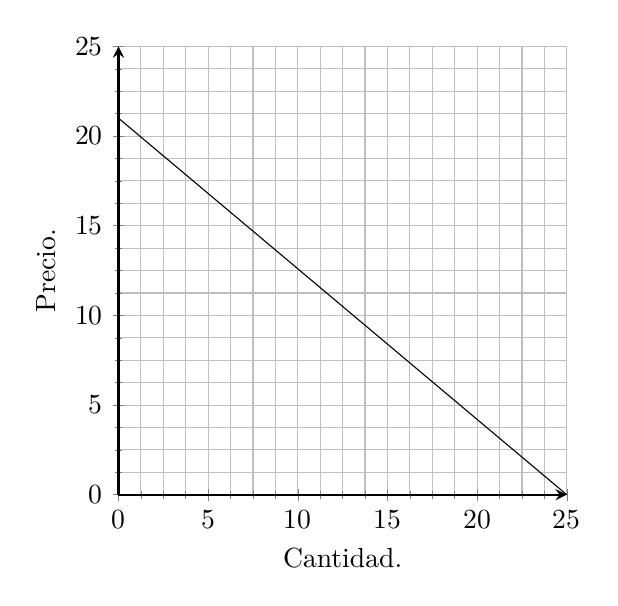
\begin{tikzpicture}
    \begin{axis}[grid=both,
    unit vector ratio*=1 1 1,
    axis x line=bottom,
    axis y line=left,
    axis line style=thick,
    xmax=25,xmin=0,
    ymax=25,ymin=0,
    xtick={0,5,10,15,20,25},
    ytick={0,5,10,15,20,25},
    minor tick num=3,
    xlabel=Cantidad.,
    ylabel=Precio.,
    ylabel near ticks,
    ylabel style={align=center},
    xlabel near ticks,
    ]
    
    \addplot[draw, smooth] coordinates {(0,21) (25,0)};
    \end{axis}
    \end{tikzpicture}
\end{center}

\end{multicols}

~ Como se puede ver, mientras más cantidad hay, menos demanda hay. Por
lo que el precio demandado baja.

\hypertarget{equilibrio-de-mercado}{%
\section{Equilibrio de mercado:}\label{equilibrio-de-mercado}}

~ Cuando el valor de la demanda y de la oferta son iguales, significa
que hay equilibrio de mercado. Esto se puede ver en la intersección de
ambas curvas en un gráfico.

~ Si decimos que los dos gráficos anteriores son del mismo bien entonces
el gráfico del equilibrio de mercado sería:

\begin{center}
    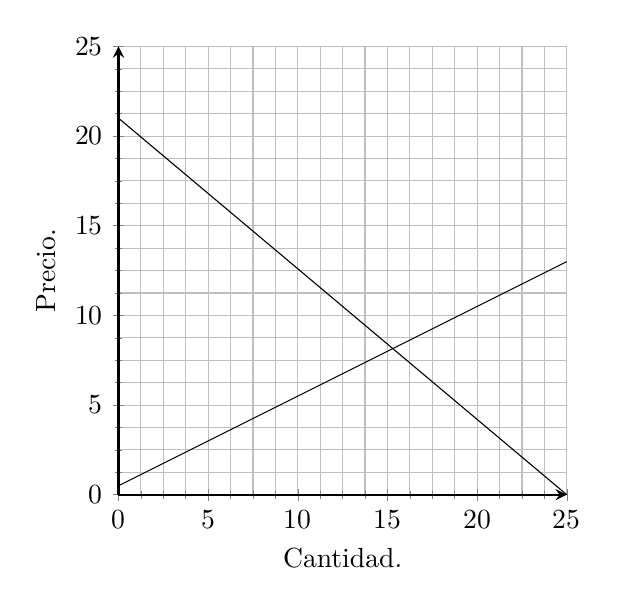
\begin{tikzpicture}
    \begin{axis}[grid=both,
    unit vector ratio*=1 1 1,
    axis x line=bottom,
    axis y line=left,
    axis line style=thick,
    xmax=25,xmin=0,
    ymax=25,ymin=0,
    xtick={0,5,10,15,20,25},
    ytick={0,5,10,15,20,25},
    minor tick num=3,
    xlabel=Cantidad.,
    ylabel=Precio.,
    ylabel near ticks,
    ylabel style={align=center},
    xlabel near ticks,
    ]
 
    \addplot[draw, smooth] coordinates {(0,21) (25,0)};
    \addplot[draw, smooth] coordinates {(0,0.5) (25,13)};
    \end{axis}
    \end{tikzpicture}
\end{center}

~ El punto de intersección es cuando el precio es de \$11 y hay 12,5
unidades de producción. Este es el punto de equilibrio de mercado, si el
mercado está sobre ese punto es que hay un exceso de oferta, y su está
más bajo, es que hay escasez.

\hypertarget{cambios-de-curvas}{%
\section{Cambios de curvas:}\label{cambios-de-curvas}}

~ Podemos analizar que sucediera si hay un cambio en la curva de oferta
y demanda, los cambios se relacionan de la siguiente forma:

\begin{table}[H]
    \centering
    \begin{tabular}{|p{25mm}|p{25mm}|p{25mm}|p{25mm}|p{25mm}|}
        \hline
         & Sin cambio en la oferta & Un incremento de la oferta & Un decremento de la oferta  \\ \hline
        Sin cambio en la oferta & P igual \par Q igual & P disminuye \par Q aumenta & P aumenta \par Q disminuye \\ \hline
        Un incremento de la oferta & P aumenta \par Q aumenta & P ambiguo \par Q aumenta & P aumenta \par Q ambiguo\\ \hline
        Un decremento de la oferta & P disminuye \par Q disminuye & P disminuye \par Q ambiguo & P ambiguo \par Q disminuye \\ \hline
    \end{tabular}
\end{table}

~ Por lo general, lo que hace que las curvas cambien de posición son
eventos bruscos, por ejemplo, en el mercado de las lecherías, si se
contamina con un antibiótico la central de ``colun'' la curva de oferta
aumentaría, ya que, es menos lo que se podría ofrecer.

~ Puede ocurrir que cambien las posiciones de ambas curvas
simultáneamente.

~ Ahora veremos cómo afecta esto en el punto de equilibrio:

~ Tomaremos como situación antes del cambio el siguiente gráfico.

\begin{center}
    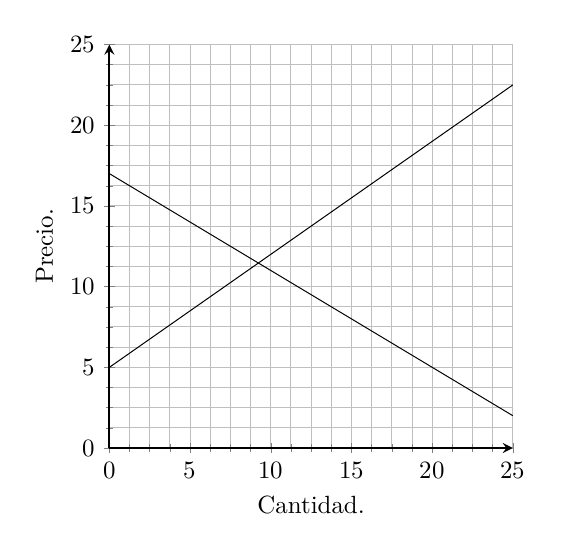
\begin{tikzpicture}[scale=0.9]
    \begin{axis}[grid=both,
    unit vector ratio*=1 1 1,
    axis x line=bottom,
    axis y line=left,
    axis line style=thick,
    xmax=25,xmin=0,
    ymax=25,ymin=0,
    xtick={0,5,10,15,20,25},
    ytick={0,5,10,15,20,25},
    minor tick num=3,
    xlabel=Cantidad.,
    ylabel=Precio.,
    ]
    \addplot [
    domain=0:25, 
    samples=100, 
    color=black,
    ]
    {5+0.7*x};
    \addplot [
    domain=0:25, 
    samples=100, 
    color=black,
    ]
    {17-0.6*x};
    \end{axis}
    \end{tikzpicture}
\end{center}

~ Los siguientes gráficos representan el cambio:

\begin{multicols}{2}
\begin{center}
    \indent Curva de oferta se desplaza hacia la izquierda:
    
    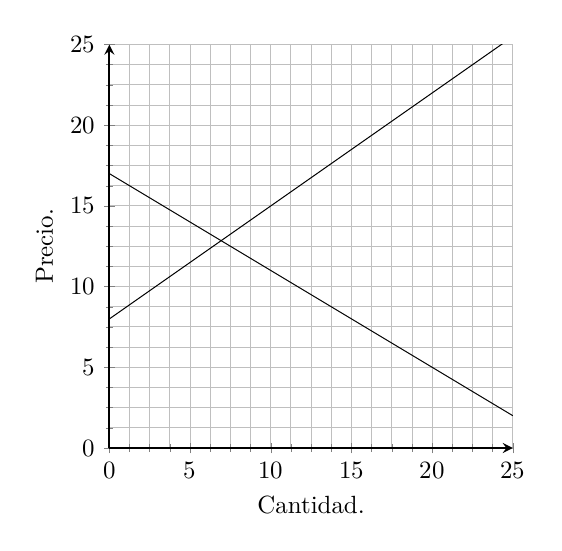
\begin{tikzpicture}[scale=0.9]
    \begin{axis}[grid=both,
    unit vector ratio*=1 1 1,
    axis x line=bottom,
    axis y line=left,
    axis line style=thick,
    xmax=25,xmin=0,
    ymax=25,ymin=0,
    xtick={0,5,10,15,20,25},
    ytick={0,5,10,15,20,25},
    minor tick num=3,
    xlabel=Cantidad.,
    ylabel=Precio.,
    ]
    \addplot [
    domain=0:25, 
    samples=100, 
    color=black,
    ]
    {8+0.7*x};
    \addplot [
    domain=0:25, 
    samples=100, 
    color=black,
    ]
    {17-0.6*x};
    \end{axis}
    \end{tikzpicture}
\end{center}

\begin{center}
    \indent Curva de demanda e desplaza hacia la derecha:
    
    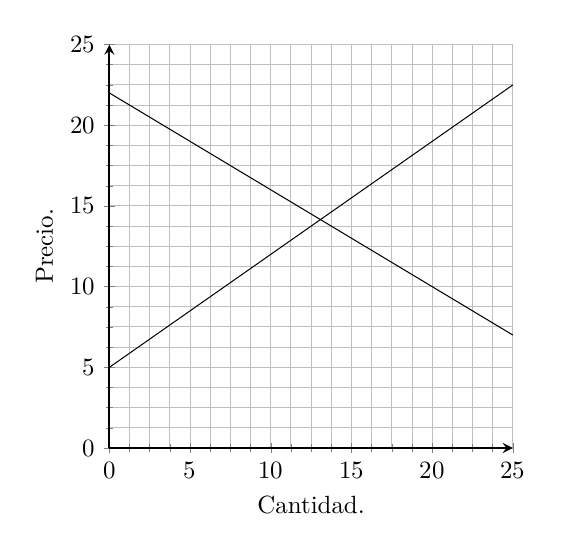
\begin{tikzpicture}[scale=0.9]
    \begin{axis}[grid=both,
    unit vector ratio*=1 1 1,
    axis x line=bottom,
    axis y line=left,
    axis line style=thick,
    xmax=25,xmin=0,
    ymax=25,ymin=0,
    xtick={0,5,10,15,20,25},
    ytick={0,5,10,15,20,25},
    minor tick num=3,
    xlabel=Cantidad.,
    ylabel=Precio.,
    ]
    \addplot [
    domain=0:25, 
    samples=100, 
    color=black,
    ]
    {5+0.7*x};
    \addplot [
    domain=0:25, 
    samples=100, 
    color=black,
    ]
    {22-0.6*x};
    \end{axis}
    \end{tikzpicture}
\end{center}

\end{multicols}

\newpage

\begin{multicols}{2}

\begin{center}
    \indent Curva de oferta e desplaza hacia la derecha:
    
    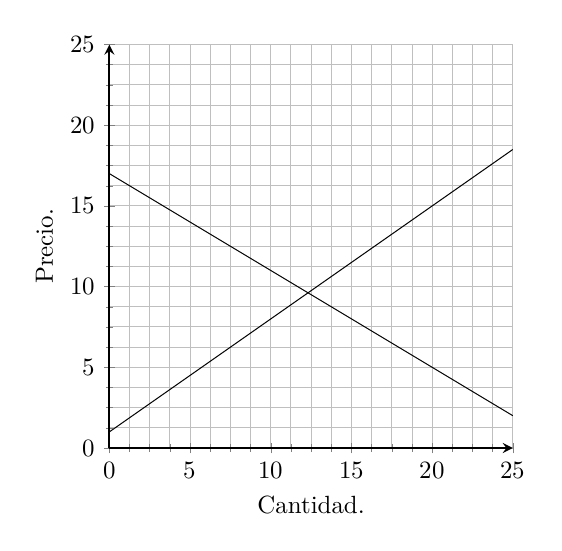
\begin{tikzpicture}[scale=0.9]
    \begin{axis}[grid=both,
    unit vector ratio*=1 1 1,
    axis x line=bottom,
    axis y line=left,
    axis line style=thick,
    xmax=25,xmin=0,
    ymax=25,ymin=0,
    xtick={0,5,10,15,20,25},
    ytick={0,5,10,15,20,25},
    minor tick num=3,
    xlabel=Cantidad.,
    ylabel=Precio.,
    ]
    \addplot [
    domain=0:25, 
    samples=100, 
    color=black,
    ]
    {1+0.7*x};
    \addplot [
    domain=0:25, 
    samples=100, 
    color=black,
    ]
    {17-0.6*x};
    \end{axis}
    \end{tikzpicture}
\end{center}
 
\begin{center}
    \indent Curva de demanda e desplaza hacia la izquierda:
    
    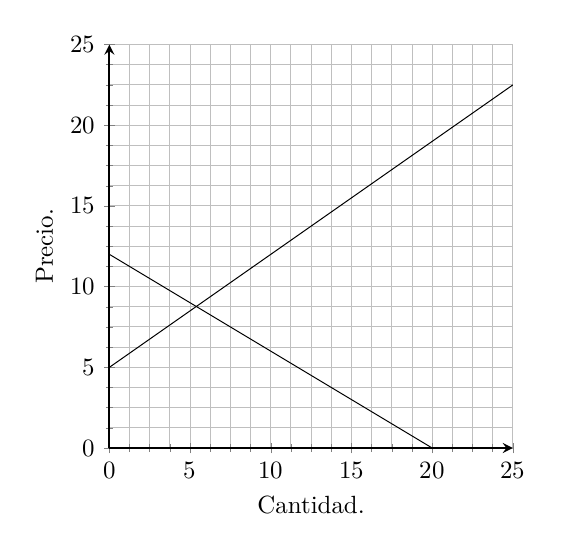
\begin{tikzpicture}[scale=0.9]
    \begin{axis}[grid=both,
    unit vector ratio*=1 1 1,
    axis x line=bottom,
    axis y line=left,
    axis line style=thick,
    xmax=25,xmin=0,
    ymax=25,ymin=0,
    xtick={0,5,10,15,20,25},
    ytick={0,5,10,15,20,25},
    minor tick num=3,
    xlabel=Cantidad.,
    ylabel=Precio.,
    ]
    \addplot [
    domain=0:25, 
    samples=100, 
    color=black,
    ]
    {5+0.7*x};
    \addplot [
    domain=0:25, 
    samples=100, 
    color=black,
    ]
    {12-0.6*x};
    \end{axis}
    \end{tikzpicture}
\end{center}

\end{multicols}

\hypertarget{elasticidad}{%
\section{Elasticidad:}\label{elasticidad}}

~ La elasticidad de la oferta y la demanda se calcula con esta fórmula:
\[
\in =\left|\frac{\triangle\%Q}{\triangle\%P} \right|
\] ~ Donde \(\in\) es la elasticidad, \(\triangle\%\) el cambio
porcentual, Q es la demanda y P el precio.

\[
f(x)= \left\{ \begin{array}{lcc}
     \text{Inelástica} &   \text{si}  & \in < 1 \\
     \\ \text{Absolutamente inelástica} &  \text{si} & \in = 0 \\
     \\ \text{Elasticidad unitaria} &  \text{si}  & \in = 1 \\
     \\ \text{Elástica} &  \text{si}  & \in > 1
     \end{array}
\right.
\]

~ \ul{Ejercicio resuelto:}

~ Tenemos las siguientes expresiones \(P_1(Q)\) y \(P_2(Q)\) que son la
ecuación de oferta hace un año y de ahora respectivamente y \(P_3(Q)\) y
\(P_4(Q)\) que son la ecuación de demanda de hace un año y actual,
calcule y clasifique su elasticidad.

\[
\begin{matrix}
    P_1(Q)=10+4Q &  P_2(Q)=30+4Q \\
    P_3(Q)=310-6Q & P_4(Q)=200-6Q \\
\end{matrix}
\]

~ \textbf{Respuesta:}

~ \ul{Paso I: encontrar el equilibrio de mercado del antes y el ahora.}

~ Equilibrio antiguo:

\[
10+4Q=310-6Q \Leftrightarrow 300=10Q \Leftrightarrow Q=30
\]

\[
P_3(Q)=310-6 \cdot 30 \Leftrightarrow P_3 = P_1 = 130
\]

\[
(30,130)
\]

~ Equilibrio actual:

\[
30+4Q=200-6Q \Leftrightarrow 170=10Q \Leftrightarrow Q=17
\]

\[
P_2(Q)=30+4 \cdot 17 \Leftrightarrow P_2 = P_4 = 98
\]

\[
(17,98)
\]

~ \ul{Paso II: Calcular la elasticidad y clasificarla.}

\[
\in =\left|\dfrac{1-\frac{17}{30}}{1-\frac{98}{130}} \right|
\]

\[
\in =\dfrac{\frac{13}{30}}{\frac{32}{130}}
\]

\[
\in =\dfrac{1690}{960}
\]

\[
\in =1,7604
\]

~ Es elástica.

\bookmarksetup{startatroot}

\hypertarget{intervenciones-del-mercado.}{%
\chapter{Intervenciones del
mercado.}\label{intervenciones-del-mercado.}}

\hypertarget{economuxeda-de-bienestar}{%
\section{Economía de bienestar:}\label{economuxeda-de-bienestar}}

~ La economía de bien estar se basa en la disposición de un comprador a
pagar o un productor a producir. Por lo que se puede ver desde el punto
de vista del oferente y del demandante:

~ En el siguiente gráfico veremos de forma clara la representación de
ambos puntos de vista:

\begin{figure}

{\centering \includegraphics[width=0.6\textwidth,height=\textheight]{3interverción_files/figure-pdf/unnamed-chunk-1-1.pdf}

}

\end{figure}

~ Donde
\texttt{EC\textquotesingle{}\textquotesingle{}\ es\ el\ excedente\ del\ consumidor\ y}EP'\,'
es el excedente del productor.

~ \textbf{Excedente del consumidor:}

~ Se calcula como el precio que está dispuesto a pagar el consumidor
menos lo que paga. De forma puntual se puede formular como: \[
ec = p_c - P_e
\]

~ Donde \(ec\) es el excedente de un consumidor especifico, \(p_c\) es
el precio máximo dispuesto a pagar y \(P_e\) el precio en el equilibrio.

~ De forma general es el área marcada con naranjo en el gráfico, pero
también lo puedes calcular con la siguiente formula. \[
EC = \int_{0}^{Q_e}{P_d(Q)-P_e \ dQ}
\]

~ Donde ``\(P_e\)'' es el precio de equilibrio y ``\(Q_0\)'', es la
cantidad en el equilibrio.

~ \textbf{Excedente del productor:}

~ De forma general es el área marcada con naranjo en el gráfico, pero
también lo puedes calcular con la siguiente formula. \[
EC = \int_{0}^{Q_e}{P_e-P_s(Q) \ dQ}
\]

\hypertarget{intervenciuxf3n-del-gobierno}{%
\section{Intervención del
gobierno:}\label{intervenciuxf3n-del-gobierno}}

~ Las intervenciones estatales son cambios forzados que hace el gobierno
a un mercado, estos generan una pérdida de eficiencia, también llamada
\textbf{peso muerto}, esto hace que cambien las decisiones de las
personas.

~ Una de las formas de intervención del gobierno es agregar por ley un
\textbf{precio máximo}, este es el precio máximo legal, y también puede
agregar un \textbf{precio mínimo} que es el precio mínimo legal. Si el
precio máximo esta por sobre el equilibrio no influye en el mercado,
pero si esta por debajo, genera escasez. Por otro lado, si el precio
mínimo esta por debajo del equilibrio, no influye en el mercado. Por el
contrario, si esta sobre el equilibrio genera superávit.

~ Para que el gobierno se financie, les agrega un impuesto a los
productos que hará subir el costo y precio de estos, dicho de otra forma
el excedente del consumidor y productor disminuye, y ambos pagan la
misma cantidad de impuesto al comprar o vender ese producto.

~ También existen otras intervenciones del estado, como, por ejemplo, el
subsidio, se le conoce como el impuesto negativo, ya que, el consumidor
paga menos. Igual que los impuestos, pero de forma contraría, la
financiación del estado es repartido equitativamente entre los
participantes de ese mercado.

~ Los siguientes gráficos son posibles ejemplos de ambas situaciones.
Donde,
\texttt{O\ mer\textquotesingle{}\textquotesingle{}\ es\ oferta\ sin\ impuesto\ o\ subsidio,}D
mer'\,' es demanda sin impuesto o subsidio, el área negra es la perdida
de eficiencia o peso muerto, ``GOB'\,' es lo que recibe o financia el
gobierno, dependiendo si es impuesto o subsidio respectivamente y EC y
EP son los excedentes del consumidor y productor respectivamente.

\begin{multicols}{2}

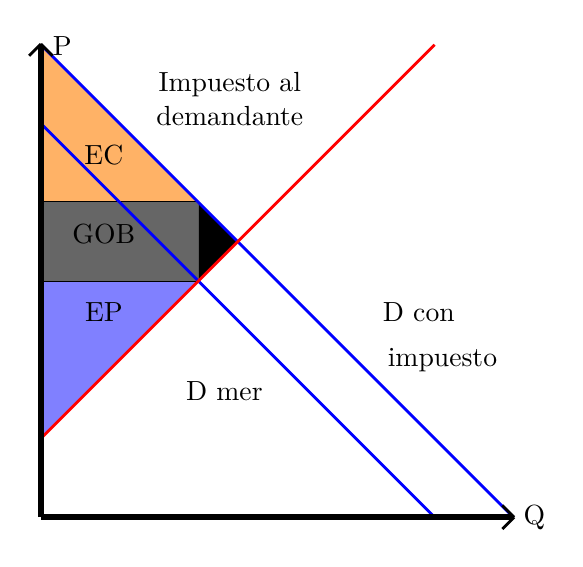
\begin{tikzpicture}

    % oferta = P(Q)=1+Q
    % demanda libre = P(Q)=5-Q
    % demanda con impuesto = 6-Q
    
    
    % Etiquetas en el eje P
    % Area excedente del consumidor
    \fill[orange!60] (0,4) -- (2,4) -- (0,6) -- cycle;
    \draw [line width=1pt](0,4) -- (2,4);
    
    % Area excedente del productor
    \fill[blue!50] (0,3) -- (2,3) -- (0,1) -- cycle;
    \draw [line width=1pt](0,3) -- (2,3);
    
    % Area de impuesto recuadado.
    \fill[black!60] (0,4) -- (2,4) -- (2,3) -- (0,3)-- cycle;
    
    % perdida de eficiencia.
    \fill[black] (2,3) -- (2,4) -- (2.5,3.5) -- cycle;
    
    % demanda sin impuesto
    \draw [blue, line width=1pt](0,5) -- (5,0); %P(Q)=5-Q

    %demanda con impuesto
    \draw [blue, line width=1pt](0,6) -- (6,0);

    % oferta
    \draw [red, line width=1pt](0,1) -- (5,6); %P(Q)=1+Q
       
    % Eje x
    \draw[black, line width=2pt] (0,0) -- (5.98,0) node[right] {Q};
    \draw[black, line width=1pt] (5.86,-0.15) -- (6.01,0);
    \draw[black, line width=1pt] (5.86,0.15) -- (6.01,0);

    % eje y
    \draw[black, line width=2pt] (0,0) -- (0,5.98) node[right] {P};
    \draw[black, line width=1pt] (-0.15,5.86) -- (0,6.01);
    \draw[black, line width=1pt] (0.15,5.86) -- (0,6.01);

    %leyendas
    \node at (0.8,2.6) {EP};
    \node at (0.8,4.6) {EC};
    \node at (0.8,3.6) {GOB};
    \node at (4.8,2.6) {D con};
    \node at (5.1,2) {impuesto};
    \node at (2.33,1.6) {D mer};
    \node at (2.4,5.5) {Impuesto al};
    \node at (2.4,5.1) {demandante};
    
\end{tikzpicture}

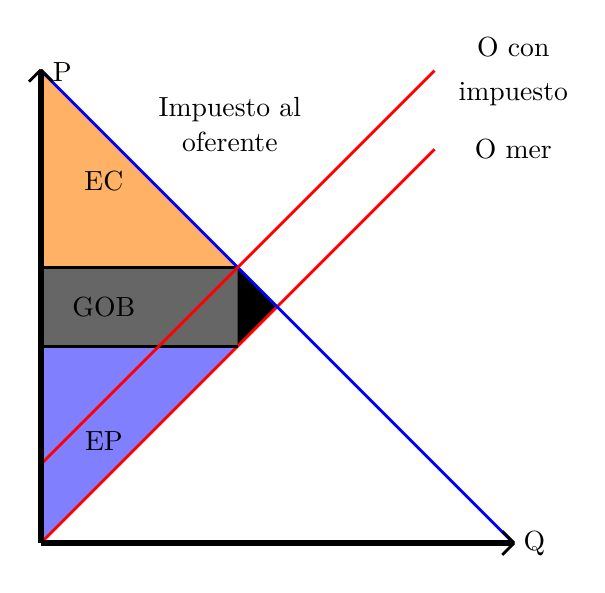
\begin{tikzpicture}

    % oferta = P(Q)=1+Q
    % demanda libre = P(Q)=5-Q
    % demanda con impuesto = 6-Q
    
    
    % Etiquetas en el eje P
    % Area excedente del consumidor
    \fill[orange!60] (0,3.5) -- (2.5,3.5) -- (0,6) -- cycle;
    
    % Area excedente del productor
    \fill[blue!50] (0,2.5) -- (2.5,2.5) -- (0,0) -- cycle;
    
    % Area de impuesto recuadado.
    \fill[black!60] (0,2.5) -- (0,3.5) -- (2.5,3.5) -- (2.5,2.5)-- cycle;
    
    % perdida de eficiencia.
    \fill[black] (2.5,3.5) -- (2.5,2.5) -- (3,3) -- cycle;
    
    % oferta sin impuesto
    \draw [red, line width=1pt](0,0) -- (5,5); %P(Q)=5-Q
    \draw [line width=1pt](0,2.5) -- (2.5,2.5);
    \draw [line width=1pt](0,3.5) -- (2.5,3.5);

    %demanda con impuesto
    \draw [blue, line width=1pt](0,6) -- (6,0);

    % oferta
    \draw [red, line width=1pt](0,1) -- (5,6); %P(Q)=1+Q
    
    % Eje x
    \draw[black, line width=2pt] (0,0) -- (5.98,0) node[right] {Q};
    \draw[black, line width=1pt] (5.86,-0.15) -- (6.01,0);
    \draw[black, line width=1pt] (5.86,0.15) -- (6.01,0);

    % eje y
    \draw[black, line width=2pt] (0,0) -- (0,5.98) node[right] {P};
    \draw[black, line width=1pt] (-0.15,5.86) -- (0,6.01);
    \draw[black, line width=1pt] (0.15,5.86) -- (0,6.01);

    %leyendas
    \node at (0.8,1.3) {EP};
    \node at (0.8,4.6) {EC};
    \node at (0.8,3) {GOB};
    \node at (6,6.3) {O con};
    \node at (6,5.7) {impuesto};
    \node at (6,5) {O mer};
    \node at (2.4,5.5) {Impuesto al};
    \node at (2.4,5.1) {oferente};
    
\end{tikzpicture}

\end{multicols}

\begin{multicols}{2}

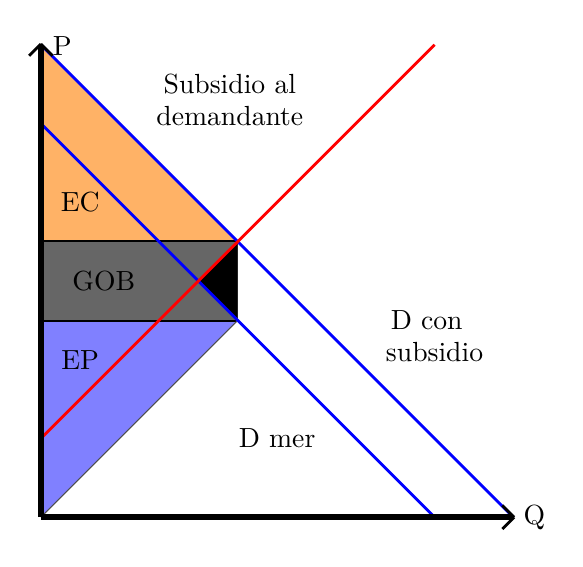
\begin{tikzpicture}

    % oferta = P(Q)=1+Q
    % demanda libre = P(Q)=5-Q
    % demanda con subsidio = 4-Q
    
    
    % Etiquetas en el eje P
    % Area excedente del consumidor
    \fill[orange!60] (0,3.5) -- (2.5,3.5) -- (0,6) -- cycle;
    \draw [line width=1pt](0,3.5) -- (2.5,3.5);
    
    % Area excedente del productor
    \fill[blue!50] (0,2.5) -- (2.5,2.5) -- (0,0) -- cycle;
    \draw [line width=1pt](0,2.5) -- (2.5,2.5);
    \draw [black!70](0,0) -- (2.5,2.5);
    
    % Area de impuesto recuadado.
    \fill[black!60] (0,2.5) -- (0,3.5) -- (2.5,3.5) -- (2.5,2.5)-- cycle;
    
    % perdida de eficiencia.
    \fill[black] (2,3) -- (2.5,2.5) -- (2.5,3.5) -- cycle;
    
    % demanda sin subsidio
    \draw [blue, line width=1pt](0,5) -- (5,0); %P(Q)=5-Q

    %demanda con subsidio
    \draw [blue, line width=1pt](0,6) -- (6,0);

    % oferta
    \draw [red, line width=1pt](0,1) -- (5,6); %P(Q)=1+Q
    
    % Eje x
    \draw[black, line width=2pt] (0,0) -- (5.98,0) node[right] {Q};
    \draw[black, line width=1pt] (5.86,-0.15) -- (6.01,0);
    \draw[black, line width=1pt] (5.86,0.15) -- (6.01,0);

    % eje y
    \draw[black, line width=2pt] (0,0) -- (0,5.98) node[right] {P};
    \draw[black, line width=1pt] (-0.15,5.86) -- (0,6.01);
    \draw[black, line width=1pt] (0.15,5.86) -- (0,6.01);

    %leyendas
    \node at (0.5,2) {EP};
    \node at (0.5,4) {EC};
    \node at (0.8,3) {GOB};
    \node at (4.9,2.5) {D con};
    \node at (5,2.1) {subsidio};
    \node at (3,1) {D mer};
    \node at (2.4,5.5) {Subsidio al};
    \node at (2.4,5.1) {demandante};
    
\end{tikzpicture}

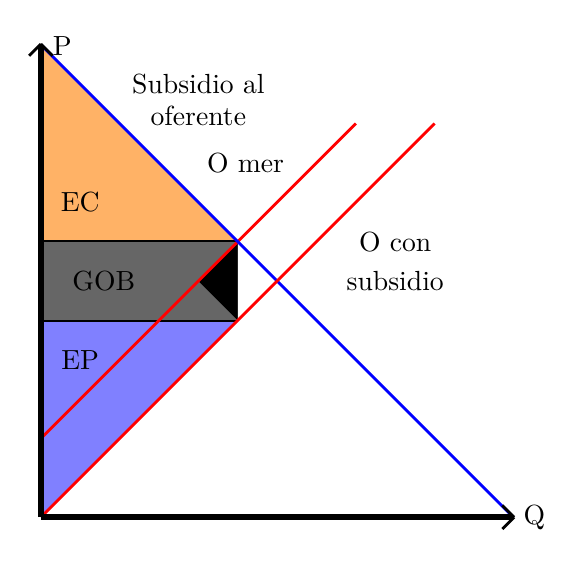
\begin{tikzpicture}

    % oferta = P(Q)=1+Q
    % demanda libre = P(Q)=5-Q
    % demanda con subsidio = 4-Q
    
    
    % Etiquetas en el eje P
    % Area excedente del consumidor
    \fill[orange!60] (0,3.5) -- (2.5,3.5) -- (0,6) -- cycle;
    \draw [line width=1pt](0,3.5) -- (2.5,3.5);
    
    % Area excedente del productor
    \fill[blue!50] (0,2.5) -- (2.5,2.5) -- (0,0) -- cycle;
    \draw [line width=1pt](0,2.5) -- (2.5,2.5);
    
    % Area de subsidio recuadado.
    \fill[black!60] (0,2.5) -- (0,3.5) -- (2.5,3.5) -- (2.5,2.5)-- cycle;
    
    % perdida de eficiencia.
    \fill[black] (2.5,2.5) -- (2.5,3.5) -- (2,3) -- cycle;
    
    % oferta sin subsidio
    \draw [red, line width=1pt](0,1) -- (4,5); %P(Q)=5-Q

    %demanda
    \draw [blue, line width=1pt](0,6) -- (6,0);

    % oferta
    \draw [red, line width=1pt](0,0) -- (5,5); %P(Q)=1+Q
    
    % Eje x
    \draw[black, line width=2pt] (0,0) -- (5.98,0) node[right] {Q};
    \draw[black, line width=1pt] (5.86,-0.15) -- (6.01,0);
    \draw[black, line width=1pt] (5.86,0.15) -- (6.01,0);

    % eje y
    \draw[black, line width=2pt] (0,0) -- (0,5.98) node[right] {P};
    \draw[black, line width=1pt] (-0.15,5.86) -- (0,6.01);
    \draw[black, line width=1pt] (0.15,5.86) -- (0,6.01);

    %leyendas
    \node at (0.5,2) {EP};
    \node at (0.5,4) {EC};
    \node at (0.8,3) {GOB};
    \node at (2.6,4.5) {O mer};
    \node at (4.5,3.5) {O con};
    \node at (4.5,3) {subsidio};
    \node at (2,5.5) {Subsidio al};
    \node at (2,5.1) {oferente};
    
\end{tikzpicture}

\end{multicols}





\newpage

\begin{multicols}{2}

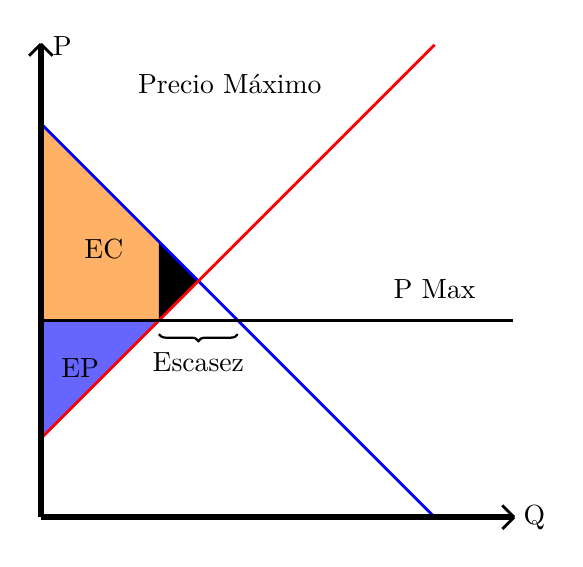
\begin{tikzpicture}

    % oferta = P(Q)=1+Q
    % demanda = P(Q)=5-Q
    
    
    % Etiquetas en el eje P
    % Area excedente del consumidor
    \fill[orange!60] (0,2.5) -- (0,5) -- (1.5,3.5) -- (1.5,2.5) -- cycle;
    
    % Area excedente del productor
    \fill[blue!60] (0,2.5) -- (1.5,2.5) -- (0,1) -- cycle;
    
    % perdida de eficiencia.
    \fill[black] (2,3) -- (1.5,3.5) -- (1.5,2.5) -- cycle;
    
    % demanda
    \draw [blue, line width=1pt](0,5) -- (5,0); %P(Q)=5-Q

    % oferta
    \draw [red, line width=1pt](0,1) -- (5,6); %P(Q)=1+Q
    
    \draw [line width=1pt](0,2.5) -- (6,2.5);
    
    % Eje x
    \draw[black, line width=2pt] (0,0) -- (5.98,0) node[right] {Q};
    \draw[black, line width=1pt] (5.86,-0.15) -- (6.01,0);
    \draw[black, line width=1pt] (5.86,0.15) -- (6.01,0);

    % eje y
    \draw[black, line width=2pt] (0,0) -- (0,5.98) node[right] {P};
    \draw[black, line width=1pt] (-0.15,5.86) -- (0,6.01);
    \draw[black, line width=1pt] (0.15,5.86) -- (0,6.01);

    %leyendas
    \node at (0.5,1.9) {EP};
    \node at (0.8,3.4) {EC};
    \draw [thick, decoration={brace, mirror, raise=5pt}, decorate] (1.5,2.5) -- (2.5,2.5) node[midway, below=8pt] {Escasez};
    \node at (5,2.9) {P Max};
    \node at (2.4,5.5) {Precio Máximo};
\end{tikzpicture}

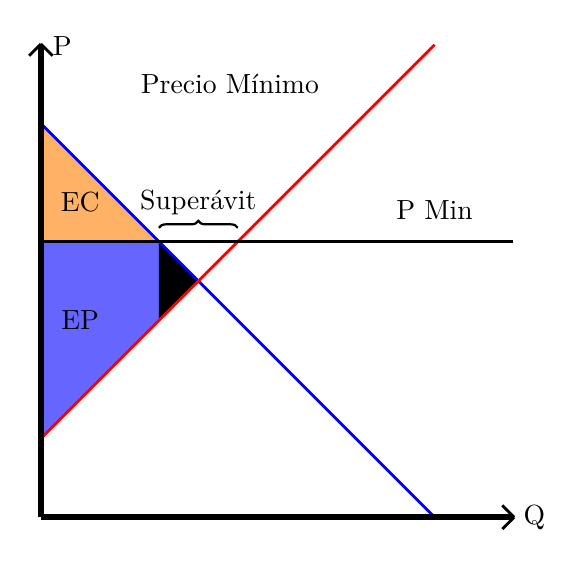
\begin{tikzpicture}

    % oferta = P(Q)=1+Q
    % demanda = P(Q)=5-Q
    
    
    % Etiquetas en el eje P
    % Area excedente del consumidor
    \fill[orange!60] (0,3.5) -- (0,5) -- (1.5,3.5) -- cycle;
    
    % Area excedente del productor
    \fill[blue!60] (0,1) -- (0,3.5) -- (1.5,3.5) -- (1.5,2.5) -- cycle;
    
    % perdida de eficiencia.
    \fill[black] (2,3) -- (1.5,3.5) -- (1.5,2.5) -- cycle;
    
    % demanda
    \draw [blue, line width=1pt](0,5) -- (5,0); %P(Q)=5-Q

    % oferta
    \draw [red, line width=1pt](0,1) -- (5,6); %P(Q)=1+Q
    
    \draw [line width=1pt](0,3.5) -- (6,3.5);
    
    % Eje x
    \draw[black, line width=2pt] (0,0) -- (5.98,0) node[right] {Q};
    \draw[black, line width=1pt] (5.86,-0.15) -- (6.01,0);
    \draw[black, line width=1pt] (5.86,0.15) -- (6.01,0);

    % eje y
    \draw[black, line width=2pt] (0,0) -- (0,5.98) node[right] {P};
    \draw[black, line width=1pt] (-0.15,5.86) -- (0,6.01);
    \draw[black, line width=1pt] (0.15,5.86) -- (0,6.01);

    %leyendas
    \node at (0.5,2.5) {EP};
    \node at (0.5,4) {EC};
    \draw [thick, decoration={brace, raise=5pt}, decorate] (1.5,3.5) -- (2.5,3.5);
    \node at (5,3.9) {P Min};
    \node at (2,4) {Superávit};
    \node at (2.4,5.5) {Precio Mínimo};
    
\end{tikzpicture}

\end{multicols}

\hypertarget{comercio-internacional}{%
\section{Comercio internacional:}\label{comercio-internacional}}

~ Existe un término que se llama \textbf{precio mundial} que hace
referencia al valor del costo de oportunidad. Esto hace que exista una
ventaja comparativa en cada país que incentiva a cada país a
especializarse en algún o algunos bienes específicos.

~ Para saber si conviene importar o exportar se hace un diagrama
agregando el precio mundial y el excedente al exportar o importar un
bien.

\& nbsp; \textbf{Exportaciones.}

~ En el caso de una economía local, que tenga un precio en el equilibrio
menor que el del precio mundial y decida exportar, tendrá un gráfico,
donde
\texttt{BE\textquotesingle{}\textquotesingle{}\ es\ el\ beneficio\ de\ exportación\ y}PM'\,'
es el precio mundial, de la siguiente manera:

\newpage

\begin{figure}

{\centering \includegraphics[width=0.5\textwidth,height=\textheight]{3interverción_files/figure-pdf/unnamed-chunk-8-1.pdf}

}

\end{figure}

~ \textbf{Importaciones.}

~ Para el caso de las importaciones sucede porque el precio de
equilibrio local es más alto que el precio mundial. Entonces, los
consumidores deciden importar. En este caso, llamaremos a ``BI'' como lo
que no se pierde por la decisión de importar.

\begin{figure}

{\centering \includegraphics[width=0.5\textwidth,height=\textheight]{3interverción_files/figure-pdf/unnamed-chunk-9-1.pdf}

}

\end{figure}

~ \textbf{Arancel:}

~ El \textbf{arancel} por su parte es un impuesto a los productos
traídos del extranjero creando que el precio de estos suba. Esto influye
en los consumidores del país, porque el valor de lo que compren va a ser
igual a la suma del arancel y el precio mundial. En el gráfico ``Ar'' lo
llamaremos arancel, el área negra será la perdida de eficiencia y
``PA'', lo que gana el gobierno por medio del arancel.

\newpage

\begin{figure}

{\centering \includegraphics[width=0.5\textwidth,height=\textheight]{3interverción_files/figure-pdf/unnamed-chunk-10-1.pdf}

}

\end{figure}

\hypertarget{consecuencias-de-la-intervenciuxf3n-en-los-participantes-de-un-mercado.}{%
\section{Consecuencias de la intervención en los participantes de un
mercado.}\label{consecuencias-de-la-intervenciuxf3n-en-los-participantes-de-un-mercado.}}

~ Como vimos en los gráficos anteriores al hacer una intervención en el
mercado, algunos participantes pueden ganar o perder excedente. Aun así,
es importante aclarar que un mercado intervenido, siempre tendrá su
dosis de ineficiencia. En las siguientes tablas veremos como afecta en
cada tipo de intervención.

\begin{table}[H]
    \centering
    \begin{tabular}{|p{45mm}|p{30mm}|p{30mm}|}
        \hline
        Intervención & Demandante & Oferente \\
        \hline
        Impuesto & Pierde excedente & Pierde excedente \\
        \hline
        Subsidio & Gana excedente & Gana excedente \\
        \hline
        Fijación precio máximo & Pierde excedente & Gana excedente \\
        \hline
        Fijación precio mínimo & Gana excedente & Pierde excedente \\
        \hline
    \end{tabular}
    \caption{Intervención I.}
    
\end{table}

~ Para el caso del comercio internacional sería de la siguiente forma:

\begin{table}[H]
    \centering
    \begin{tabular}{|p{48mm}|p{30mm}|p{30mm}|p{30mm}|}
        \hline
        Intervención & Productor local & Productor internacional. & Demandante local \\
        \hline
        Aplicar arancel o cerrarse al mercado internacional. & Gana excedente & Pierde excedente en dicho lugar & Pierde excedente \\
        \hline
        Eliminar arancel o abrirse al mercado internacional. & Pierde excedente & Gana excedente en dicho lugar & Gana excedente \\
        \hline
    \end{tabular}
    \caption{Intervención II.}
    
\end{table}

\bookmarksetup{startatroot}

\hypertarget{sistema-impositivo-y-economuxeda-laboral.}{%
\chapter{Sistema impositivo y economía
laboral.}\label{sistema-impositivo-y-economuxeda-laboral.}}

\hypertarget{financiamiento-del-gobierno}{%
\section{Financiamiento del
gobierno:}\label{financiamiento-del-gobierno}}

~ El gobierno necesita financiar sus gastos, para esto tiene dos
maneras, usar el impuesto o la deuda.

~ Si el gobierno gasta más de lo que recibe, entonces tiene un
\textbf{déficit presupuestario}, pero si gasta menos de lo que recibe
tiene un \textbf{superávit presupuestal}.

~ Los impuestos dan principalmente cargos administrativos para que la
gente cumpla las leyes fiscales.

~ Un sistema impositivo es más eficiente mientras recauda más ingreso y
mientras menos sea el costo de los contribuyentes, es decir,
equitativamente.

~ En el principio de beneficios dice que todos deben pagar sus impuestos
con respecto a los beneficios que recibe del gobierno. Mientras que el
principio de pago dice que los impuestos deben ser cobrados según dos
tipos de equidad, \textbf{Equidad horizontal:} los contribuyentes con
misma capacidad de pago pagan igual cantidad y \textbf{Equidad
vertical:} los contribuyentes con mayor capacidad de pago pagan más.

~ Los impuestos pueden ser: \textbf{proporcionales}, es decir, todos
deben pagar la misma fracción de sus ingresos, \textbf{regresivos}, los
contribuyentes con mayor ingreso deben pagar una fracción menor de su
ingreso que los con menor ingreso o \textbf{progresivos}, los
contribuyentes con menor ingreso deben pagar una fracción menor de su
ingreso que los con mayor ingreso.

~ El impuesto altera el equilibrio de precios, por lo que muchas veces
no se toma en cuenta en la decisión de estos las consecuencias
indirectas.

\hypertarget{fallas-del-mercado}{%
\section{Fallas del mercado:}\label{fallas-del-mercado}}

~ La economía de bienestar tiene una fuga al no tomar dos supuestos
importantes:

\begin{enumerate}
\def\labelenumi{\arabic{enumi}.}
\item
  \textbf{Poder de mercado:} Hay veces que existe un solo vendedor
  (monopolio) o un solo vendedor (monopsonio).
\item
  \textbf{externalidades:} Las decisiones de los compradores y
  vendedores a veces afectan a algún tercero y no paga o compensa el
  daño a este último, un ejemplo típico es la contaminación.
\end{enumerate}

~ Estas fugas se llaman \textbf{fallas de mercado} y hacen que el punto
de equilibrio no sea eficiente.

~ Hay externalidades negativas cuando valor del bien el consumido o del
bien producido es menor del que la da la sociedad.

~ \ul{Por ejemplo:}

~ La producción de jeans gasta las aguas limpias, y el consumo de autos,
consume aire puro.

~ En estas situaciones el estado puedo interceder poniendo impuestos
como incentivos, prohibiciones por decreto de ley, regulaciones como
permisos. En una situación ideal estas intervenciones estatales ayudan a
compensar el costo indirecto.

~ Esto puede ser a través de la propiedad privada, como multar a una
empresa que contamina más de lo establecido, o a través del
comportamiento privado como prohibir la caza excesiva de un animal en
peligro de extinción.

~ También pueden solucionar estos problemas los privados por el teorema
de Coase: ``si las partes pueden negociar sin costo y si los derechos
iniciales están bien definidos, entonces es posible una solución privada
y además eficiente''.

~ Los free-riders o parásitos son aquellos individuos que se benefician
d algo y no pagan los costos de aquello. Por ejemplo, dentro de un grupo
para las tareas del curso puede existir alguien que no hizo nada en el
trabajo, pero como la nota es grupal se beneficia de ello sin haber
hecho nada.

~ Dentro de los bienes que están dentro de estas fallas de mercados se
pueden clasificar de dos formas, \textbf{excluyentes} si se puede evitar
que las personas usen ese bien y si es \textbf{rival de consumo}, dicho
de otra forma, si son limitados y si alguien usa el bien reduce la
capacidad para que otro lo use también.

\begin{table}[h]
    \centering
    \begin{tabular}{|p{30mm}|p{30mm}|p{30mm}|}
        \hline
        - & Es excluyente. & No es excluyente. \\ \hline
        Es rival en consumo. & Bienes privados. \par - Ropa. \par - Teléfonos. & Recursos comunes. \par - Peces en el océano. \par -El ambiente. \\ \hline
        No es rival en consumo. & Bienes reservados. \par - Televisión por cable. \par -Protección de incendios. \par & Bienes públicos. \par - Defensa nacional. \par - Alarmas de emergencias. \\ \hline
    \end{tabular}
    
\end{table}

~ Cuando el parásito evade el costo de transacción influye en la
eficiencia de las instituciones benéficas o de bien común, como son la
defensa nacional, investigaciones y lucha contra la pobreza.

~ A la parábola que muestra como los bienes comunes se usan más de lo
que se debe, se llama \textbf{tragedia de los comunes}.

~ Con respecto al poder de mercado, existen dos tipos de monopolio:

\begin{itemize}
\tightlist
\item
  Monopolios creados por el gobierno: Generalmente, están relacionados
  con la creación de un nuevo bien, si el gobierno considera que este es
  completamente original, le dará al creador una patente para que solo
  pueda venderlo el durante un tiempo determinado.
\item
  Monopolios naturales: Si una empresa puede vender un mismo bien más
  barato porque sus costos de producción son menores, entonces tendrá
  todo el poder de mercado.
\end{itemize}

~ Al tener todo el poder de mercado, estos tienen el poder del precio de
demanda, pero no de la oferta, pongamos el caso de un empresario
benevolente que tenga todo el poder de mercado y luego, propongamos que
se corrompe y que sube los precios de tal forma que su excedente sea
mayor, para el primer caso, tendremos el siguiente gráfico de su
mercado:

\begin{figure}

{\centering \includegraphics[width=0.6\textwidth,height=\textheight]{4sistimpo_files/figure-pdf/unnamed-chunk-1-1.pdf}

}

\end{figure}

~ Luego, cuando se corrompe, se verá algo así:

\begin{figure}

{\centering \includegraphics[width=0.5\textwidth,height=\textheight]{4sistimpo_files/figure-pdf/unnamed-chunk-2-1.pdf}

}

\end{figure}

\hypertarget{curva-de-laffer}{%
\section{Curva de Laffer:}\label{curva-de-laffer}}

La curva de Laffer hace referencia a lo recaudado por el gobierno con
relación a la cantidad de impuesto agregado. Podemos verla así:

\begin{figure}

{\centering \includegraphics[width=0.5\textwidth,height=\textheight]{4sistimpo_files/figure-pdf/unnamed-chunk-3-1.pdf}

}

\end{figure}

~ El punto de máxima recaudación es el punto en que el peso muerto es
igual a la recaudación. Donde podemos decir que el peso muerto es:

\[
\text{Peso muerto}=\frac{(P_f-P_i)\cdot (Q_i-Q_f)}{2}
\]

~ Y lo recaudado por el estado es:

\[
\text{Gob}=Q_f\cdot (P_f-P_i)
\]

~ Además, \(Q_i\) y \(P_i\) son los puntos de equilibrio y los puntos
\(Q_f\) y \(P_f\) son las coordenadas del nuevo punto de equilibrio.

\hypertarget{demanda-y-oferta-de-trabajo}{%
\section{Demanda y oferta de
trabajo:}\label{demanda-y-oferta-de-trabajo}}

~ Además de la oferta y demanda en función del precio, existen por
insumos y servicios, donde la mayoría de los bienes producidos son
insumos para otros bienes, como son los chips para los autos,
computadores, sistemas de riego, etc.

~ Los insumos son tierra, trabajo y capital, por otro lado, está la
producción que depende de los insumos disponibles. Cuando se grafica
este tipo de oferta o demanda, se pone en el eje de las abscisas o de
las ``\(x\)'', los insumos y en el eje de las ordenadas, o el de las
``\(y\)'' la producción.

~ \textbf{Demanda:} en la demanda de trabajo, existe el
\textbf{``producto marginal del trabajo''}, o el incremento la cantidad
producida por unidad de trabajo adicional, esto es decreciente, esto
quiere decir, que mientras más personas se dedican a hacer un producto,
menos producirá cada persona.

~ \textbf{Oferta:} en la oferta de trabajo, muestra las decisiones de
los trabajadores entre la disyuntiva ocio y trabajo, para poder
incentivar el trabajo un recurso típico y mayoritariamente efectiva es
la subida de sueldos. Hay tres factores que mueven la curva de la oferta
de trabajo: inmigración, cambio de preferencias, cambio de oportunidades
de trabajo.

~ Ejemplificando, los dos últimos son, preferir trabajar como minero que
cosechero para el cambio de preferencias, o en el caso de querer seguir
con la especialización actual, preferir cosechar en los cerezos que en
las manzanas.

~ \textbf{Punto de equilibrio:} el punto de equilibrio hace referencia
al salario que tendrá la persona, es donde intersecan la oferta y la
demanda.

\hypertarget{determinantes-de-los-salarios-de-equilibrio}{%
\section{Determinantes de los salarios de
equilibrio:}\label{determinantes-de-los-salarios-de-equilibrio}}

~ Hay cuatro determinantes que definirán el salario de una persona:

\begin{table}[h]
    \centering
    \begin{tabular}{|p{40mm}|p{40mm}|p{40mm}|}
        \hline
        Determinante: & Explicación: & Ejemplo: \\ \hline
    Diferencial compensativo. & Es la diferenciación al compensar características no monetarias. & Turnos nocturnos. \\ \hline
    Capital humano. & Educación y capacitación para poder hacer el trabajo. & Enseñar a los lecheros como se ordeña. \\ \hline
    Educación como señal. & Según la teoría no ayuda a la producción, pero da una referencia a su capacidad para lograr hacer el trabajo. & Persona que realizo sus estudios en una buena academia para el trabajo que se busca. \\ \hline
    Suerte, esfuerzo y capacidad. & Son características innatas del trabajador, pero son difíciles de medir de forma justa. & Una persona que se levanta más temprano para ir a trabajar que otra. \\ \hline
    \end{tabular}
    
\end{table}

~ Podemos graficar la relación de producción y salario de la siguiente
forma:

\begin{figure}

{\centering \includegraphics[width=0.7\textwidth,height=\textheight]{4sistimpo_files/figure-pdf/unnamed-chunk-4-1.pdf}

}

\end{figure}

\hypertarget{diferenciaciuxf3n-de-los-salarios}{%
\section{Diferenciación de los
salarios:}\label{diferenciaciuxf3n-de-los-salarios}}

~ Un excedente de salario es cuando el salario esta por sobre del punto
de equilibrio, esto puede pasar por tercer razones: \textbf{salario
mínimo} más alto de lo que corresponde, \textbf{sindicatos} que amenazan
con huelga si no se sube el sueldo, \textbf{salarios de eficiencia} para
inducir que los trabajadores rindan más.

~ Cualquier excedente de salario implica desempleo.

~ Existen también otra diferenciación del salario, esta es la
\textbf{discriminación} ocurre cuando se les paga una cantidad distinta
a las personas de distinta etnia, raza, sexo, etc. Esta práctica sucede
tanto en sectores privados como estatales. Una empresa que quiere crecer
en su beneficio tiende a eliminar la mayor cantidad de diferenciaciones
posible.

\hypertarget{mercados-de-trabajo}{%
\section{Mercados de trabajo:}\label{mercados-de-trabajo}}

~ Antes de, definiremos un par de conceptos: - \(Q(K,L)\) es producción.
- \(K\) es capital, puede referirse al capital de añadir una maquina de
producción por ejemplo. - \(L\) es la cantidad de trabajadores. -
\(\bar{n}\) la variable de n es fija, actúa como constante.

~ Ahora, todos estos conceptos tienen otras definiciones, en la
siguiente tabla se explicarán:

\begin{table}[h]
    \centering
    \begin{tabular}{|p{40mm}|p{40mm}|p{40mm}|}
        \hline
        Medida: & Formula: & Utilidad: \\\hline
        Producto marginal del trabajo: & \[\frac{dQ(K,L)}{dL}\] & Crecimiento de producción por unidad de trabajo \\\hline
        Producto marginal del capital: & \[\frac{dQ(K,L)}{dK}\] & crecimiento de producción por unidad de capital (al agregar una maquina por ejemplo.) \\\hline
        Productividad media del trabajo: & \[\frac{Q(K,L)}{L}\] & Promedio de producción por cada trabajador \\\hline
        Productividad media del capital: & \[\frac{Q(K,L)}{K}\] & Promedio de producción por cada recurso que usa el capital. \\\hline
        Retornos de trabajo: & \[\frac{d^2Q(K,L)}{dL^2}\] & Comportamiento de producción al agregar más o menos trabajadores. \\\hline
        Retornos de capital: & \[\frac{d^2Q(K,L)}{dK^2}\] & Comportamiento de producción al agregar más o menos capital. \\\hline
    \end{tabular}
    
\end{table}

~ Los retornos de producción serán: \[
\text{Retornos} =
\begin{cases}
  \text{Constantes a escala}, & \text{si } \frac{d^2Q(L,K)}{d(L\vee K)^2} = 1 \\
  \text{Crecientes}, & \text{si } \frac{d^2Q(L,K)}{d(L\vee K)^2} > 1 \\
  \text{Decrecientes}, & \text{si } \frac{d^2Q(L,K)}{d(L\vee K)^2} < 1
\end{cases}
\]

~ \ul{Caso de ejemplo:}

~ Tenemos la siguiente función de producción:

\[
Q(K,L)=L^3+2KL^2+K^3
\]

~ Calcule todas las medidas de producción y la producción marginal del
trabajo para \(\bar{K}=5\).

~ \textbf{Respuesta:}

\begin{table}[h]
    \centering
    \begin{tabular}{|p{40mm}|p{40mm}|}
        \hline
        Medida: & Resultado\\\hline
        Producto marginal del trabajo: & \[3L^2+4KL\] \\\hline
        Producto marginal del capital: & \[2L^2+3K^2\] \\\hline
        Productividad media del trabajo: & \[L^2+2K+\frac{K^3}{L}\] \\\hline
        Productividad media del capital: & \[\frac{L^3}{K}+2L^2+K^2\] \\\hline
        Retornos de trabajo: & \[6L+4K\]  \\\hline
        Retornos de capital: & \[6K\] \\\hline
    \end{tabular}
    
\end{table}

~ Para \(\bar{K}=5\) la producción marginal del trabajo será: \[
P(L)3L^2+20L
\]

\hypertarget{uxedndice-de-pobreza}{%
\section{Índice de pobreza:}\label{uxedndice-de-pobreza}}

~ El índice de pobreza es el porcentaje de la población que su sueldo
familiar está por debajo de la \textbf{línea de pobreza}, y esta última
es el nivel establecido por el gobierno que distingue desde que punto
una familia tiene un sueldo bajo o normal.

~ \textbf{Curva de Lorenz}, es un gráfico que representa en eje
horizontal se sitúan la población en porcentaje que tiene como máximo un
sueldo y en el eje vertical el sueldo en porcentaje, en el siguiente
grafico se puede ver la curva de Lorenz.

\begin{figure}

{\centering \includegraphics[width=0.7\textwidth,height=\textheight]{4sistimpo_files/figure-pdf/unnamed-chunk-5-1.pdf}

}

\end{figure}

~ Por otro lado, está el \textbf{coeficiente de Gini:} esta muestra en
un parámetro

de \([0,1]\) el nivel de desigualdad. Donde 0 es la perfecta igualdad:
\[
G=1-\left|\sum_{k=1}^{n-1}\left(X_{k+1}-X_k\right)\left(Y_{k+1}+Y_k\right)\right| 
\]

~ Donde \(X\) es la proporción acumulada de población e \(Y\) es la
proporción acumulada de ingresos.

~ \ul{Por ejemplo:}

~ Dividiremos la población en 10 deciles con sus sueldos promedio:

\begin{table}[H]
    \centering
    \begin{tabular}{|p{25mm}|p{25mm}|}
        \multicolumn{2}{c}{Tabla de demanda:} \\
        \hline
        Percentil “$X$”: & Ingresos “$Y$”: \\ \hline
        10 & 0.02 \\ \hline
        20 & 0.03 \\ \hline
        30 & 0.04 \\ \hline
        40 & 0.06 \\ \hline
        50 & 0.08 \\ \hline
        60 & 0.1 \\ \hline
        70 & 0.12 \\ \hline
        80 & 0.14 \\ \hline
        90 & 0.17 \\ \hline
        100 & 0.24 \\ \hline
        \end{tabular}
\end{table}

~ Entonces la sumatoria resolviendo el primer decil queda así:

\[
G=1-\left|\left(0,2-0,1\right)\left(0,3+0,2\right)+\sum_{k=2}^{n-1}\left(X_{k+1}-X_k\right)\left(Y_{k+1}+Y_k\right)\right|
\]

~ Existen tres filosofías para solucionar el problema de la pobreza:

\begin{enumerate}
\def\labelenumi{\arabic{enumi})}
\tightlist
\item
  \textbf{Utilitarismo:} El gobierno decide qué medidas tomar para que
  todos aumenten sus beneficios.
\item
  \textbf{Liberalismo:} El gobierno deberá elegir políticas consideradas
  justas, evaluadas por un observador objetivo.
\item
  \textbf{Liberalismo del libre albedrio:} El gobierno debe castigar los
  crímenes y hacer velar los acuerdos voluntarios, la igualdad de
  oportunidades vale más que la igualdad en el ingreso.
\end{enumerate}

~También existen políticas para intentar reducir la pobreza: - Regular
sueldo mínimo. - Asistencia social o programas de gobierno para
complementar el ingreso. - Subsidio a hogares con bajos ingresos. -
Entregar bienes y servicios de parte del gobierno.

\bookmarksetup{startatroot}

\hypertarget{variables-macroeconuxf3micas.}{%
\chapter{Variables
macroeconómicas.}\label{variables-macroeconuxf3micas.}}

\hypertarget{producto-interno-bruto}{%
\section{Producto interno bruto:}\label{producto-interno-bruto}}

~ El producto interno bruto o PIB mide dos cosas al mismo tiempo, lo que
producen todas las personas en la economía y lo que gastan todas las
personas en la economía, existen tres tipos:

\begin{table}[h]
    \centering
    \begin{tabular}{|p{40mm}|p{40mm}|p{50mm}|}
        \hline
        PIB de corrientes o nominal: & PIB a precios constantes o real: & Deflactor del PIB: \\ \hline
        Mide la producción total de cada bien $q_{i,t}$ por sus precios $p_{i,t}$. & Mide el cambio de la producción de un bien $q_{i,0}$ por su precio con respecto a un año base $q_{i,0}$.  & Calcula el nivel de precios con el PIB nominal partido el real. \\ \hline
        \[Y=\sum{q_{i,t}p_{i,t}}\] & \[y=\sum{q_{i,0}p_{i,0}}\] & \[Def \, PIB =\frac{PIB\ nominal}{PIB\ real}\] \\ \hline
    \end{tabular}
    
\end{table}

~ El PIB se puede medir de tres formas:

\begin{itemize}
\tightlist
\item
  Por el lado del gasto: \(Y=C+I+G+X+M\).
\item
  Por el lado del producto: con la matriz insumo-producto.
\item
  Por el lado de los ingresos: hogares son dueños de factores
  productivos.
\end{itemize}

\hypertarget{crecimiento-del-pib}{%
\section{Crecimiento del PIB:}\label{crecimiento-del-pib}}

\begin{table}[h]
    \centering
    \begin{tabular}{|p{55mm}|p{75mm}|}
        \hline
        PIB real & PIB nominal \\ \hline
        Considera cambio de precios y cantidades a través del tiempo t. & Solo considera el cambio los cambios en cantidades a través del tiempo t. \\ \hline
        \[\mathrm{\Delta}\%{PIB}_t=\frac{{PIB}_t-{PIB}_{t-1}}{{PIB}_{t-1}}\] & \[\textrm{infalción}_t=\frac{Deflactor_t-Deflactor_{t-1}}{Deflactor_{t-1}}\]  \\ \hline
    \end{tabular}
    
\end{table}

\hypertarget{otros-medidores}{%
\section{Otros medidores:}\label{otros-medidores}}

~ \textbf{IMACEC:} el índice mensual de actividad económica es otro
medidor que incluye el \(90\%\) de los bienes y servicios del PIB.

~ \textbf{IPC:} el índice de precios al consumidor es la medida del
costo total de bienes y servicios de un consumidor promedio. Para
calcularlo se necesitan hacer los siguientes pasos: 1) Fijar la canasta:
lo que consume un consumidor promedio. 2) Encontrar los precios de los
bienes de la canasta. 3) Calcular los costos de la canasta. 4) Elegir un
año base y calcular el índice con la siguiente formula: \[
\text{IPC}=\frac{\text{Precio de la canasta actual}}{\text{Precio de la canasta del año base}}
\]

~ El problema del IPC es que a veces sobreestima los valores de la
canasta o agrega bienes que pueden ser innecesario y también que no mide
la calidad de la canasta. Aun así, podemos medir la inflación con esta
medida:

\[
\text{Infalción}_t=\frac{IPC_t-IPC_{t-1}}{IPC_{t-1}}
\]

~ Para poder mantener un precio real sobre un bien o servicio se
\textbf{indexa}, la indexación es dar un precio que no le afecta la
inflación, como, por ejemplo, las UTM, la UF, etc.

~ La UF o unidad de fomento es un índice que se ajusta todos los días
con respecto a la inflación, para que algunos contractos no se
desvaloricen.

\hypertarget{desempleo}{%
\section{Desempleo:}\label{desempleo}}

\begin{figure}[H]

{\centering \includegraphics[width=6.16in,height=4.28in]{5varia_files/figure-latex/mermaid-figure-1.png}

}

\end{figure}

~ Existen dos tipos de desempleo: - \textbf{Friccional:} la persona
busca un trabajo que se adapte a sus gustos y necesidades. -
\textbf{Estructural:} por pocos empleos disponibles es imposible darle
empleo a todos los que necesiten uno.

~ Para mantener a la persona cesante con un ingreso durante un tiempo
existe un seguro de desempleo, está dado por ley que cuando se firma un
contrato se tiene que estar afiliado automáticamente a ese seguro.

\hypertarget{otros-factores-de-la-producciuxf3n}{%
\section{Otros factores de la
producción:}\label{otros-factores-de-la-producciuxf3n}}

~ Para que una sociedad tenga una alta calidad de vida se necesitan
producir bienes y servicios, dicho de otra forma, se necesita
\textbf{productividad}. Y para tener productividad se necesita:

\begin{table}[H]
    \centering
    \begin{tabular}{|p{30mm}|p{90mm}|}
        \hline
        Capital humano: & Capacidades de los trabajadores en hacer un trabajo gracias a su educación y especialización. \\ \hline
        Capital físico: & Conjunto de equipos y estructuras que se necesitan para producir. \\ \hline
        Recursos naturales: & Los da la naturaleza, son cosas como minerales, ríos, tierra. \\ \hline
        Conocimiento tecnológico: & Comprensión de la mejor forma en que la sociedad puede producir un bien. \\ \hline
    \end{tabular}
    
\end{table}

~ Para incrementar la producción se tiene que invertir en recursos
naturales, pero de forma coherente con las necesidades y posibilidades
de las personas. Por esta misma razón el rendimiento del capital es
decreciente, por esta razón, es más fácil para un país pobre mejorar
económicamente que para uno rico. A esto se le llama \textbf{efecto
convergencia}.

~ Los países con bajo capital humano tienen diferencias grandes
salariales, pero para la producción es mejor invertir en educación,
porque tienen mejor especialización y luego tendrán más salarios para
poder estar más sanos, un trabajador enfermo produce menos que uno sano.

\bookmarksetup{startatroot}

\hypertarget{introducciuxf3n-a-las-finanzas.}{%
\chapter{Introducción a las
finanzas.}\label{introducciuxf3n-a-las-finanzas.}}

\hypertarget{finanzas-y-riesgos}{%
\section{Finanzas y riesgos:}\label{finanzas-y-riesgos}}

~ La \textbf{finanza} es el área de estudio que analiza como las
personas toman decisiones en asignar valor a un recurso, comprarlo y
venderlo a través del tiempo, con una medida de riesgo, ya que, los
bienes pueden valorizarse o desvalorizarse.

~ Para eso está el \textbf{valor presente} que es la cantidad de dinero
del presente que se necesita para producir determinada cantidad de
dinero en el futuro.

~ El \textbf{valor futuro} que es la cantidad de dinero en el futuro que
se necesitara para producir la cantidad de dinero hoy.

~ Y por último está el \textbf{valor compuesto} que es la acumulación de
dinero a través del tiempo, más la suma del interés agregado a través
del tiempo. La fórmula del dinero acumulado es así:

\[
VF=\left(1+i\right)VP
\]

~ Para poder enfrentar un riesgo de forma más tranquila se tiende a
comprar un seguro, donde se reparten las perdidas. Los seguros enfrentan
ciertas dificultades como:

\begin{enumerate}
\def\labelenumi{\arabic{enumi})}
\item
  \textbf{Selección adversa:} las personas que compran este seguro
  generalmente tienden ser los que más arriesgan.
\item
  \textbf{Riesgo moral:} las personas con este seguro tienen menos
  incentivos a ser cuidadosas con su dinero.
\end{enumerate}

~ Otra forma de poder invertir de forma menos arriesgada es la
diversificación, esto es invertir en distintos bienes o servicios. Esta
puede eliminar el riesgo especifico de empresas que se tiene
incertidumbre, pero no elimina el riesgo del mercado.

~ Hay una relación entre riesgo y rendimiento, donde si arriesgo más
puedo ganar más, pero también puedo perder más.

\hypertarget{valorizaciuxf3n-de-las-empresas}{%
\section{Valorización de las
empresas:}\label{valorizaciuxf3n-de-las-empresas}}

~ Para valorizar una empresa se le pide a un estudio de \textbf{análisis
fundamental} que le de valor a su empresa y sus \textbf{acciones}, este
último es una parte de la empresa, por lo que, si existen 100 acciones
de una empresa, la persona que tenga una acción es dueña del \(1\%\) de
la empresa.

~ El análisis que hace el estudio de análisis fundamental se llama
portafolio de acciones, donde el sueño de la empresa puede aceptar su
valor, hacer por sí solo el análisis o comprar un fondo de inversiones
con un administrador donde el administrador lo analice y tome las
decisiones.

~ En un principio los valores de la oferta y demanda determinan el valor
de estas acciones, pero a veces la gente puede creer que vale más
haciendo que suban de precio creando una \textbf{burbuja de
especulación} cuando revientan es cuando nadie más compra, al suceder
eso se desvaloriza su valor.

\bookmarksetup{startatroot}

\hypertarget{ejercicios-propuestos}{%
\chapter{Ejercicios propuestos:}\label{ejercicios-propuestos}}

\hypertarget{sobre-capuxedtulo-i}{%
\section{Sobre capítulo I:}\label{sobre-capuxedtulo-i}}

\hypertarget{section}{%
\subsection{:}\label{section}}

\begin{enumerate}
\def\labelenumi{\arabic{enumi})}
\tightlist
\item
  A causa de las constantes enfermedades pulmonares y riesgos para la
  salud, el gobierno decide aumentar el impuesto al tabaco. Como
  consecuencia de esto, un 37\% de los fumadores deja este vicio y hay
  un 45\% menos de enfermedades relacionadas al uso de esta ¿Qué
  principio esta relacionado con este cambio económico?
\item
  Dado que bajaron las enfermedades y que el estado logró recaudar más
  dinero por el aumento del impuesto anterior, el gobierno decide
  aumentar más aún el impuesto a este bien de consumo. Esta vez, aumento
  el mercado negro de este servicio y junto a esto, el estado recaudó
  menos y por la mala calidad del tabaco traficado aumento un \%15 las
  enfermedades relacionadas a este habito. ¿Qué principio es el que esta
  relacionado con este nuevo cambió?
\item
  Ahora, un comprador cualquiera de cigarrillos al ver que subieron los
  impuestos, tiene que decidir entre comprar una cajetilla o comprar la
  revista que compra todos los domingos ¿Que principio es el que se
  relaciona a esta situación?
\end{enumerate}

\hypertarget{section-1}{%
\subsection{:}\label{section-1}}

~ Con respecto al modelo de economía circular. 1) ¿Qué demandan los
hogares? 2) ¿Qué demandan las empresas? 3) ¿Qué ofrecen los hogares? 4)
¿Qué ofrecen las empresas?

\hypertarget{section-2}{%
\subsection{:}\label{section-2}}

~ Tenemos que un pastelero tiene como insumo limitante 100 huevos, para
hacer un pie de limón gasta 10 huevos, mientras que para hacer un kg de
pan gasta 5 huevos. 1) si quiere hacer 3 pie de limón, cuanto es la
máxima cantidad de pan que puede hacer. 2) exprese la situación en la
forma matemática \(\bar x=a_1y_1+a_2y_2\). 3) Haga un gráfico de la
situación. 4) Ahora, digamos que le llegaron más huevos y le alcanzó
para hacer 15 pie de limón y 15 kg de pan, cuantos huevos más tiene.

\hypertarget{section-3}{%
\subsection{:}\label{section-3}}

~ Un productor ``\(A\)'' de chocolate tiene como factor limitante el
cacao, si quiere producir chocolate dulce necesita ``\(c\)'' de este
bien por cada kg y si quiere producir chocolate amargo necesita
``\(d\)'' de este bien por cada kg. Para gastar todo su cacao necesita
producir ``\(e\)'' kg de chocolate dulce y ``\(f\)'' de chocolate
amargo.

\begin{enumerate}
\def\labelenumi{\arabic{enumi})}
\tightlist
\item
  Haga la ecuación que represente kas FPP.
\item
  Haga el gráfico de esta ecuación.
\end{enumerate}

\hypertarget{sobre-capuxedtulo-ii}{%
\section{Sobre capítulo II:}\label{sobre-capuxedtulo-ii}}

\hypertarget{section-4}{%
\subsection{:}\label{section-4}}

\begin{enumerate}
\def\labelenumi{\arabic{enumi})}
\item
  Calcule el precio Demandado (\(P\)) de un bien para una producción de
  5 unidades (\(Q=5\)). Usted sabe que si no se producen unidades el
  precio demandado es de \$5000. Adicionalmente, usted sabe que la
  función de demanda es lineal de la forma: \(P(Q)=a-250Q\)
\item
  Calcule la función inversa de demanda para \(P(Q)=a-bQ\)
\item
  Asuma una función de demanda igual a \(P(Q)=a-235Q\). Si Usted sabe
  que 10 unidades se valoran a un precio de 7650, ¿Cuál sería el precio
  de referencia si no se produce nada?
\end{enumerate}

\#\#\#: ~ Grafique las siguientes demandas:

\begin{enumerate}
\def\labelenumi{\arabic{enumi})}
\item
  \[
  P(Q)=\$10 - 1Q
  \]
\item
  \[
  P(Q)=\$12 - 2Q
  \]
\item
  \[
  P(Q)=\$50 - 2.5Q
  \]
\end{enumerate}

\newpage

\hypertarget{section-5}{%
\subsection{:}\label{section-5}}

Calcule la función demanda de los siguiente gráficos. 1)

\begin{figure}

{\centering \includegraphics[width=0.6\textwidth,height=\textheight]{7ej_propuestos_files/figure-pdf/unnamed-chunk-1-1.pdf}

}

\end{figure}

\newpage

\begin{enumerate}
\def\labelenumi{\arabic{enumi})}
\setcounter{enumi}{1}
\tightlist
\item
\end{enumerate}

\begin{figure}

{\centering \includegraphics[width=0.6\textwidth,height=\textheight]{7ej_propuestos_files/figure-pdf/unnamed-chunk-2-1.pdf}

}

\end{figure}

\newpage

\begin{enumerate}
\def\labelenumi{\arabic{enumi})}
\setcounter{enumi}{2}
\tightlist
\item
\end{enumerate}

\begin{figure}

{\centering \includegraphics[width=0.6\textwidth,height=\textheight]{7ej_propuestos_files/figure-pdf/unnamed-chunk-3-1.pdf}

}

\end{figure}

\hypertarget{section-6}{%
\subsection{:}\label{section-6}}

~ Tenemos una empresa forestal con las siguientes funciones de demanda y
oferta: \[
P_d(Q)=100-3Q
\] \[
P_o(Q)=60+2Q
\]

~ Por causas naturales una de los cultivos se incendiaron, dejando como
nuevo punto de equilibrio \((4,88)\). Haga un gráfico del caso luego del
evento y calcule la elasticidad.

\hypertarget{sobre-el-capuxedtulo-iii}{%
\section{Sobre el capítulo III:}\label{sobre-el-capuxedtulo-iii}}

\hypertarget{section-7}{%
\subsection{:}\label{section-7}}

~ Una empresa de dulces tiene como función de oferta: \(P(Q)=1+Q\) Y
como función de demanda: \(P(Q)=5-Q\), se le agrega un impuesto al
productor de \$1, calcule su peso muerto, el excedente al consumidor, lo
recaudado por el gobierno y haga un gráfico de la situación.

\hypertarget{section-8}{%
\subsection{:}\label{section-8}}

~ Tenemos una empresa de computadores con función de demanda
\(P_d(Q)=30-3Q\) y de oferta \(P(Q)=5+2Q\), debido a la pandemia se hace
un subsidio de \$6 a los estudiantes para que puedan conectarse a sus
clases. Haga un gráfico de la situación y calcule el excedente del
productor y del consumidor.

\hypertarget{section-9}{%
\subsection{:}\label{section-9}}

~ Argentina por razones populistas, antes de las elecciones decidido
fijar los precios de algunos bienes. A base de esto en un pueblo
imaginario tiene el mercado del queso como funciones de oferta y demanda
respectivamente \(P(Q)=1.5+0.5Q\) y \(Q(P)=5-P\). La fijación al precio
máximo de este bien es de \$2. ¿Qué fenómeno ocurrirá debido a esta
intervención? Haga un gráfico de la situación.

\hypertarget{section-10}{%
\subsection{:}\label{section-10}}

~ China tiene un mercado de chips con las siguientes funciones de oferta
y demanda, con \(P\) en dolares: \[
P(Q)=120+6Q \, Q(P)=50-0.125P
\]

~ Si el precio mundial es de \$300 y este país decide exportar ¿Cuanto
es lo que tendrá de beneficio este país en dolares por la exportación.
Grafíque la situación.

\hypertarget{section-11}{%
\subsection{:}\label{section-11}}

~ El merado se zapatos en chile esta dado por las funciones de oferta y
demanda en dolares y unidades: \[
\begin{array}{cc}P(Q)=5+1.5Q, & Q(P)=5.2-\frac{2}{5}P\\\end{array}
\]

~ Además, el precio mundial de estos zapatos es de \$5 por unidad y se
tiene un arancel de \$1.

~ Grafique la situación, calcule el excedente del productor local, el
peso muerto y prediga que pasaría para los consumidores y productores
locales si se quita este arancel.

\hypertarget{sobre-capuxedtulo-iv}{%
\section{Sobre capítulo IV:}\label{sobre-capuxedtulo-iv}}

\hypertarget{section-12}{%
\subsection{:}\label{section-12}}

~ Reconozca la externalidad y su tipo, es decir, si es positiva o
negativa, en los siguientes casos y proponga en que caso podría ser
bueno aplicar un impuesto o un subsidio.

\begin{enumerate}
\def\labelenumi{\arabic{enumi})}
\tightlist
\item
  Una empresa de textiles sintéticos que da una alta taza de empleo en
  la zona contamina las aguas de los ríos cercanos. \textbackslash{}
\item
  Una empresa forestal imaginaria de monocultivo en la provincia del
  Malleco erosiona los suelos, esta produce un 15\% del PIB nominal de
  Chile. \textbackslash{}
\item
  Un criadero de caballos usados para deportes nacionales amansa a las
  crías en conjunto a una clínica que usa a estos para terapia.
  \textbackslash{}
\item
  Una fundación para ancianos tiene una buena administración, pero no
  tiene los suficientes recursos para calefacción. \textbackslash{}
\end{enumerate}

\hypertarget{section-13}{%
\subsection{:}\label{section-13}}

~ Para un mercado de libros tenemos las siguientes funciones de oferta y
demanda:

\[
\begin{array}{cc} P(Q)=5+2Q & Q(P)=15-P\\\end{array}
\]

~ Calcule cuanto es la máxima recaudación posible teniendo en cuenta la
curva de Laffer.

\hypertarget{section-14}{%
\subsection{:}\label{section-14}}

~ Defina con sus palbras los siguintes terminos: 1) Déficit
presupuestario: 2) Superávit presupuestal: 3) Equidad horizontal: 4)
Equidad vertical: 5) Impuestos proporcionales: 6) Impuestos regresivos:
7) Impuestos progresivos:

\hypertarget{section-15}{%
\subsection{:}\label{section-15}}

~ Un mercado no regulado, está constituido por un solo productor y
varios compradores, tiene de funciones de oferta y demanda \(P(Q)=1+Q\)
y \(P(Q)=5-Q\) respectivamente. El productor se corrompió y decidió
aprovecharse del mercado y obtener el máximo beneficio posible. ¿Cuánto
será su excedente?

\hypertarget{section-16}{%
\subsection{:}\label{section-16}}

~ Una empresa tiene la siguiente función de producción: \[
Q(K,L)=K^3+2K^2+KL^2+L^3
\]

~ En el mercado de la empresa, cada unidad producida es vendida por \$3
dólares.

\begin{enumerate}
\def\labelenumi{\arabic{enumi})}
\item
  Determine la función de la producción media de trabajo.
\item
  Determine la función del producto marginal del capital.
\item
  Asuma un \(\bar{K}=1\) y una cantidad de trabajadores \(\bar{L}=2\)
  ¿Cuánto es el retorno del trabajo?
\end{enumerate}

\hypertarget{section-17}{%
\subsection{:}\label{section-17}}

~ Tenemos la siguiente tabla que representa el porcentaje de población
acumulado de la población según su ingreso porcentual acumulado:

\begin{table}[H]
    \centering
    \begin{tabular}{|p{25mm}|p{25mm}|}
        \multicolumn{2}{c}{Tabla de demanda:} \\
        \hline
        decil: & Ingresos: \\ \hline
        0.1 & 0.01 \\ \hline
        0.2 & 0.02 \\ \hline
        0.3 & 0.03 \\ \hline
        0.4 & 0.06 \\ \hline
        0.5 & 0.1 \\ \hline
        0.6 & 0.15 \\ \hline
        0.7 & 0.28 \\ \hline
        0.8 & 0.39 \\ \hline
        0.9 & 0.5 \\ \hline
        1 & 1 \\ \hline
        \end{tabular}
\end{table}

\begin{enumerate}
\def\labelenumi{\arabic{enumi})}
\item
  Calcule la desigualdad con el coeficiente de Gini.
\item
  Grafique la curva de Lorenz.
\end{enumerate}

\hypertarget{section-18}{%
\subsection{:}\label{section-18}}

~ Tenemos la siguiente función de producción:
{[}Q(K,L)=7K\textsuperscript{2L}3-3K\^{}3L{]}

\begin{enumerate}
\def\labelenumi{\arabic{enumi})}
\item
  Calcule las siguientes medidas de forma genérica y calcule según el
  tipo de media la utilidad si cada producción vale \$2 dolares o el
  tipo de retorno evaluándolas con \(\bar{K}=1\) y un \(\bar{L}=2\):
\item
  ¿Para qué valor de \(L\), con \(\bar{K}=2\) el retorno de capital es
  una constante a escala?
\end{enumerate}

\hypertarget{sobre-capuxedtulo-vi}{%
\section{Sobre capítulo VI:}\label{sobre-capuxedtulo-vi}}

\hypertarget{section-19}{%
\subsection{:}\label{section-19}}

~ En Loompalandia tienen las siguientes producciones totales de los
distintos mercados en los distintos años, todo evaluados en su nueva
moneda wonkas
(\texttt{wk\textquotesingle{}\textquotesingle{})\ y\ su\ cantidad\ en\ unidades\ (}u'\,'),
admeás su producción fue siempre la misma, es decir la misma cantidad:

\begin{table}[h]
    \centering
    \begin{tabular}{|c|c|c|c|c|}
        \hline
        Bien de consumo: & 2016 & 2017 & 2018 & 2019 \\\hline
        Producción de cacao: & 2u, 100wk & 2u, 98wk & 2u, 102wk & 2u, 100wk \\\hline
        Venta de azúcar importado: & 1u, 33wk & 7u, 12wk & 15u, 22wk & 26u, 25wk\\\hline
        Producción de caramelos: & 4u, 11wk & 3u, 17wk & 5u, 19wk & 4u, 21wk\\\hline
        Venta de envoltorios de Reino Unido: & 3u, 3wk & 3u, 3wk & 3u, 2wk & 4u, 3wk\\\hline
        Producción de chicle: & 6u, 33wk & 6u, 37wk & 5u, 39wk & 6u, 44wk\\\hline
        Producción de turrones: & 4u, 78wk & 5u, 81wk & 5u, 88wk & 5u, 98wk\\\hline
        Venta de plátano local: & 7u, 10wk & 8u, 12wk & 8u, 15wk & 9u, 18wk\\\hline
    \end{tabular}
\end{table}

\begin{enumerate}
\def\labelenumi{\arabic{enumi})}
\tightlist
\item
  Calcule le inflación anual, con año base 2016, de los años 2017, 2018
  y 2019.
\item
  Si un umpalumpa pone a deposito a plazo 100 wonkas con un interes del
  20\% en el año 2016 hasta el año 2019 e indexamos su valor al los
  wonkas del año 2016 ¿Cuántos wonkas tiene?
\end{enumerate}

\hypertarget{section-20}{%
\subsection{:}\label{section-20}}

~ Con los datos del banco mundial y el SII, pudimos elaborar la
siguiente tabla:

::: \{.content-visible when-format=``pdf''\}

\begin{table}[h]
    \centering
    \begin{tabular}{|c|c|c|c|c|}
        \hline
        Año & Inflación anual & Conversión enero & Conversión enero & Conversión enero \\
        & de Angola & 1UF a CLP & 1US a CLP & 1US a KZ \\\hline
        $2018$ & $19,8\%$ & $\$26800$ & $\$640$ & $253$Kz. \\\hline
        $2019$ & $17,1\%$ & $\$27565$ & $\$703$ & $365$Kz. \\\hline
        $2020$ & $22,3\%$ & $\$28310$ & $\$793$ & $578$Kz. \\\hline
        $2021$ & $25,8\%$ & $\$29070$ & $\$760$ & $631$Kz. \\\hline
        $2022$ & No influye en el ejercicio & $\$31000$ & \$$873$ & $460$Kz. \\\hline
    \end{tabular}
    
\end{table}

::: \{.content-visible when-format=``html''\}

\begin{longtable}[]{@{}lllll@{}}
\toprule\noalign{}
\endhead
\bottomrule\noalign{}
\endlastfoot
Año & Inflación anual de Angola & Conversión enero 1UF a CLP &
Conversión enero 1US a CLP & Conversión enero 1US a KZ \\
2018 & \$19,8\textbackslash\%\$ & \$\textbackslash\$26800\$ &
\$\textbackslash\$640\$ & \$253\$Kz. \\
2019 & \$17,1\textbackslash\%\$ & \$\textbackslash\$27565\$ &
\$\textbackslash\$703\$ & \$365\$Kz. \\
2020 & \$22,3\textbackslash\%\$ & \$\textbackslash\$28310\$ &
\$\textbackslash\$793\$ & \$578\$Kz. \\
2021 & \$25,8\textbackslash\%\$ & \$\textbackslash\$29070\$ &
\$\textbackslash\$760\$ & \$631\$Kz. \\
2022 & No influye en el ejercicio & \$\textbackslash\$31000\$ &
\$\textbackslash\$873\$ & \$460\$Kz. \\
\end{longtable}

~ Usted decide el 2018 poner a deposito a plazo por cuatro años un
millón de Kwanzas angoleñas a un banco que da una tasa de interés del
20\% anual.

\begin{enumerate}
\def\labelenumi{\arabic{enumi})}
\item
  ¿Cuántas kwansas tendrás al terminar los 4 años?
\item
  ¿Cuánto es la inflación acumulada en los 4 años?
\item
  Si antes del deposito a plazo tenias los kwansas en UF e indexamos a
  UF lo invertido al terminar los 4 años ¿Cuántos UF teníamos al
  principio y al final?
\item
  ¿De qué sirvió indexar a UF al principio y al final? ¿Por qué tomamos
  la referencia de la ganancia o perdida en UF y no en la inflación de
  Angola?
\end{enumerate}

\bookmarksetup{startatroot}

\hypertarget{ejercicios-pauta}{%
\chapter{Ejercicios Pauta:}\label{ejercicios-pauta}}

\hypertarget{sobre-capuxedtulo-i-1}{%
\section{Sobre capítulo I:}\label{sobre-capuxedtulo-i-1}}

\hypertarget{section-21}{%
\subsection{:}\label{section-21}}

\begin{enumerate}
\def\labelenumi{\arabic{enumi})}
\tightlist
\item
  A causa de las constantes enfermedades pulmonares y riesgos para la
  salud, el gobierno decide aumentar el impuesto al tabaco. Como
  consecuencia de esto, un 37\% de los fumadores deja este vicio y hay
  un 45\% menos de enfermedades relacionadas al uso de esta ¿Qué
  principio esta relacionado con este cambio económico?
\item
  Dado que bajaron las enfermedades y que el estado logró recaudar más
  dinero por el aumento del impuesto anterior, el gobierno decide
  aumentar más aún el impuesto a este bien de consumo. Esta vez, aumento
  el mercado negro de este servicio y junto a esto, el estado recaudó
  menos y por la mala calidad del tabaco traficado aumento un \%15 las
  enfermedades relacionadas a este habito. ¿Qué principio es el que esta
  relacionado con este nuevo cambió?
\item
  Ahora, un comprador cualquiera de cigarrillos al ver que subieron los
  impuestos, tiene que decidir entre comprar una cajetilla o comprar la
  revista que compra todos los domingos ¿Que principio es el que se
  relaciona a esta situación?
\end{enumerate}

~ \textbf{RESPUESTA}:

\begin{enumerate}
\def\labelenumi{\arabic{enumi})}
\tightlist
\item
  ``En ocasiones, el gobierno puede mejorar los resultados del
  mercado.'' Ya que, al eliminar una externalidad negativa (un efecto
  negativo del mercado hacia la sociedad) está dando buenos resultados
  en el mercado. Dicho de otra forma, está mejorando la distribución de
  los bienes.
\item
  ``Normalmente, los mercados son un buen mecanismo de asignación de
  recursos.'' Al empeorar la situación sanitaria de la sociedad, a a
  través, de la intervención estatal, podemos concluir que en este caso,
  era mejor que el mercado no se intrevenga más.
\item
  En este caso, los principios 1,2 hacen efecto en este evento, y
  dependiendo del caso, el 4 también hace efecto. Para el primer
  principio el comprador tiene que decidir entre una cosas o otra, para
  el segundo tendrá que renunciar a una de las dos y para el cuarto en
  el caso que escoja la revista, el impuesto dado es un incentivo que
  afecta el mercado.
\end{enumerate}

\hypertarget{section-22}{%
\subsection{:}\label{section-22}}

~ Con respecto al modelo de economía circular. 1) ¿Qué demandan los
hogares? 2) ¿Qué demandan las empresas? 3) ¿Qué ofrecen los hogares? 4)
¿Qué ofrecen las empresas?

~ \textbf{RESPUESTA:}

~ Al demandar, decimos que este agente es el que quiere el bien o
servicio. Por otro lado, al ofrecer, decimos que el agente es el dueño
de este y que lo esta ofreciendo a cambio de algo.

\begin{enumerate}
\def\labelenumi{\arabic{enumi})}
\tightlist
\item
  Los hogares demandan bienes y servicios.
\item
  La empresa demanda factores de producción, es decir, trabajo, capital,
  tierra y tecnología.
\item
  los hogares ofrecen factores de producción.
\item
  las empresas ofrecen bienes y servicios.
\end{enumerate}

\hypertarget{section-23}{%
\subsection{:}\label{section-23}}

~ Tenemos que un pastelero tiene como insumo limitante 100 huevos, para
hacer un pie de limón gasta 10 huevos, mientras que para hacer un kg de
pan gasta 5 huevos. 1) si quiere hacer 3 pie de limón, cuanto es la
máxima cantidad de pan que puede hacer. 2) exprese la situación en la
forma matemática \(\bar x=a_1y_1+a_2y_2\). 3) Haga un gráfico de la
situación. 4) Ahora, digamos que le llegaron más huevos y le alcanzó
para hacer 15 pie de limón y 15 kg de pan, cuantos huevos más tiene.

~ \textbf{RESPUESTA:}

\begin{enumerate}
\def\labelenumi{\arabic{enumi})}
\tightlist
\item
  Podemos expresar esto como:
\end{enumerate}

\[
100=3\cdot 10 +5 \cdot x
\]

~ Donde ``\(x\)'' será la cantidad de pan. ~ Resolviendo:

\[
100-30= 5 \cdot x
\] \[
70/5= x
\] \[
14= x
\]

~ Se podrán hacer 14Kg de pan. 2) Esto lo podemos expresar como:

\[
100=10\cdot y_1+ 5\cdot y_2
\]

~ Donde ``\(y_1\)'' son la cantidad de pie de limón y ``\(y_2\)'' la
cantidad de huevo. 3) Calculando la máxima cantidad de pan y pies que se
pueden hacer podemos decir que el máximo de pan es \(20\) y de pies son
\(10\). El gráfico resulta:

\begin{figure}

{\centering \includegraphics[width=0.6\textwidth,height=\textheight]{8ej_pauta_files/figure-pdf/unnamed-chunk-1-1.pdf}

}

\end{figure}

\begin{enumerate}
\def\labelenumi{\arabic{enumi})}
\setcounter{enumi}{3}
\tightlist
\item
  Modelamos la ecuación, recuerde que dice cuantos huevos más tenemos,
  por lo que el resultado de la cantidad de huevos totales habrá que
  restarle los 100 iniciales. \[
  \bar x=10\cdot 15+ 5\cdot 15
  \] \[
  \bar x=150+ 75
  \] \[
  \bar x=225
  \]
\end{enumerate}

~ Ahora, a este resultado le restaremos los \(100\) huevos iniciales.

\[
\text{huevos agregados}=225-100
\] \[
\text{huevos agregados}=125
\]

\hypertarget{section-24}{%
\subsection{:}\label{section-24}}

~ Un productor ``\(A\)'' de chocolate tiene como factor limitante el
cacao, si quiere producir chocolate dulce necesita ``\(c\)'' de este
bien por cada kg y si quiere producir chocolate amargo necesita
``\(d\)'' de este bien por cada kg. Para gastar todo su cacao necesita
producir ``\(e\)'' kg de chocolate dulce y ``\(f\)'' de chocolate
amargo.

\begin{enumerate}
\def\labelenumi{\arabic{enumi})}
\tightlist
\item
  Haga la ecuación que represente kas FPP.
\end{enumerate}

\textbf{RESPUESTA}

~ Primero definimos \(y_1\) es el chocolate dulce, y el amargo es
\(y_2\), luego: \[
\bar{x}=cy_1+dy_2
\]

~ Por la segunda parte del enunciado tenemos que: \[
\bar{x}=ec+df
\]

~ Finalmente: \[
ec+df=cy_1+dy_2
\]

\begin{enumerate}
\def\labelenumi{\arabic{enumi})}
\setcounter{enumi}{1}
\tightlist
\item
  Haga el gráfico de esta ecuación.
\end{enumerate}

\textbf{RESPUESTA}

\begin{figure}

{\centering \includegraphics[width=0.6\textwidth,height=\textheight]{8ej_pauta_files/figure-pdf/unnamed-chunk-2-1.pdf}

}

\end{figure}

\hypertarget{sobre-capuxedtulo-ii-1}{%
\section{Sobre capítulo II:}\label{sobre-capuxedtulo-ii-1}}

\hypertarget{section-25}{%
\subsection{:}\label{section-25}}

\begin{enumerate}
\def\labelenumi{\arabic{enumi})}
\tightlist
\item
  Calcule el precio Demandado (\(P\)) de un bien para una producción de
  5 unidades (\(Q=5\)). Usted sabe que si no se producen unidades el
  precio demandado es de \$5000. Adicionalmente, usted sabe que la
  función de demanda es lineal de la forma: \[P(Q)=a-250Q\]
\end{enumerate}

~ \textbf{RESPUESTA}

~ Tenemos que en el caso \(Q=0\) el valor de \(P(Q)=a=5000\), entonces
con esto tenemos la función:

\[
P(Q)=5000-250Q
\]

~ Ahora evaluamos \(P(5)\) y esto nos da: \[
P(5)=5000-250\cdot 5
\] \[
P(5)=5000-1250
\] \[
P(5)=3750
\]

\begin{enumerate}
\def\labelenumi{\arabic{enumi})}
\setcounter{enumi}{1}
\tightlist
\item
  Calcule la función inversa de demanda para \(P(Q)=a-bQ\)
\end{enumerate}

~ \textbf{RESPUESTA}

~ La función inversa de la demanda es la función inversa de \(Q(P)\),
por lo que la función inversa de \(P(Q)=ab-bQ\) es esta misma.

\begin{enumerate}
\def\labelenumi{\arabic{enumi})}
\setcounter{enumi}{2}
\tightlist
\item
  Asuma una función de demanda igual a \(P(Q)=a-235Q\). Si Usted sabe
  que 10 unidades se valoran a un precio de 7650, ¿Cuál sería el precio
  de referencia si no se produce nada?
\end{enumerate}

~ \textbf{RESPUESTA}

~ El precio de referencia cuando no se produce nada es en este caso el
valor de ``\(a\)'\,', para calcularlo tenemos que plantear la ecuación
del enunciado:

\[
7650=a-235\cdot 10
\] \[
7650=a-2350
\]

\[
7650+2350=a
\] \[
a=10000
\]

~ Es decir el precio de referencia es equivalente a \$10.000.

\newpage

\hypertarget{section-26}{%
\subsection{:}\label{section-26}}

~ Grafique las siguientes demandas:

\begin{enumerate}
\def\labelenumi{\arabic{enumi})}
\tightlist
\item
  \[
  P(Q)=\$10 - 1Q
  \]
\end{enumerate}

\begin{figure}

{\centering \includegraphics[width=0.6\textwidth,height=\textheight]{8ej_pauta_files/figure-pdf/unnamed-chunk-3-1.pdf}

}

\end{figure}

\newpage

\begin{enumerate}
\def\labelenumi{\arabic{enumi})}
\setcounter{enumi}{1}
\tightlist
\item
  \[
  P(Q)=\$12 - 2Q
  \]
\end{enumerate}

\begin{figure}

{\centering \includegraphics[width=0.6\textwidth,height=\textheight]{8ej_pauta_files/figure-pdf/unnamed-chunk-4-1.pdf}

}

\end{figure}

\newpage

\begin{enumerate}
\def\labelenumi{\arabic{enumi})}
\setcounter{enumi}{2}
\tightlist
\item
  \[
  P(Q)=\$50 - 2.5Q
  \]
\end{enumerate}

\begin{figure}

{\centering \includegraphics[width=0.6\textwidth,height=\textheight]{8ej_pauta_files/figure-pdf/unnamed-chunk-5-1.pdf}

}

\end{figure}

\newpage

\hypertarget{section-27}{%
\subsection{:}\label{section-27}}

Calcule la función demanda de los siguiente gráficos. 1)

\begin{figure}

{\centering \includegraphics[width=0.6\textwidth,height=\textheight]{8ej_pauta_files/figure-pdf/unnamed-chunk-6-1.pdf}

}

\end{figure}

\[
P(Q)=5-0.2Q
\]

\newpage

\begin{enumerate}
\def\labelenumi{\arabic{enumi})}
\setcounter{enumi}{1}
\tightlist
\item
\end{enumerate}

\begin{figure}

{\centering \includegraphics[width=0.6\textwidth,height=\textheight]{8ej_pauta_files/figure-pdf/unnamed-chunk-7-1.pdf}

}

\end{figure}

\[
P(Q)=20-3Q
\]

\newpage

\begin{enumerate}
\def\labelenumi{\arabic{enumi})}
\setcounter{enumi}{2}
\tightlist
\item
\end{enumerate}

\begin{figure}

{\centering \includegraphics[width=0.6\textwidth,height=\textheight]{8ej_pauta_files/figure-pdf/unnamed-chunk-8-1.pdf}

}

\end{figure}

\[
P(Q)=10-2Q
\]

\hypertarget{section-28}{%
\subsection{:}\label{section-28}}

~ Tenemos una empresa forestal con las siguientes funciones de demanda y
oferta: \[
P_d(Q)=100-3Q
\] \[
P_o(Q)=60+2Q
\]

~ Por causas naturales una de los cultivos se incendiaron, dejando como
nuevo punto de equilibrio \((4,88)\). Haga un gráfico del caso luego del
evento y calcule la elasticidad.

~ \textbf{RESPUESTA}

~ Primero calculamos el punto de equilibrio inicial:

\[
100-3Q=60+2Q
\] \[
40=5Q
\] \[
8
\]

Reemplazamos en \(P(Q)\): \[
P(8)=100-3\cdot 8
\]

\[
P = 76
\]

~ Entonces el punto inicial es \((8,76)\). Además, al ser un evento que
le afecta a la oferta, ya que, los que demandan demandan lo mismo, pero
los que ofrecen, ofrecen menos, tendremos un cambio en la curva de
demanda.

Ahora calcularemos la nueva oferta:

\[
88=a+2\cdot 4
\]

\[
88=a+8 \Leftrightarrow a=80
\]

\[
P_o(Q)=80+2Q
\]

~ Finalmente hacemos el gráfico:

\begin{figure}

{\centering \includegraphics[width=0.6\textwidth,height=\textheight]{8ej_pauta_files/figure-pdf/unnamed-chunk-9-1.pdf}

}

\end{figure}

~ Ahora calcularemos la elasticidad:

~ Recordemos que la elasticidad es:

\[
\in =\left|\dfrac{\triangle\%Q}{\triangle\%P} \right|
\]

~ Entonces tenemos: \[
\in=\left|\frac{88-76}{8-4} \right|
\] \[
\in=\left|\frac{12}{4} \right|
\] \[
\in=3
\]

~ De esto podemos decir que es elástica.

\hypertarget{sobre-el-capuxedtulo-iii-1}{%
\section{Sobre el capítulo III:}\label{sobre-el-capuxedtulo-iii-1}}

\hypertarget{section-29}{%
\subsection{:}\label{section-29}}

~ Una empresa de dulces tiene como función de oferta: \(P(Q)=1+Q\) Y
como función de demanda: \(P(Q)=5-Q\), se le agrega un impuesto al
productor de \$1, calcule su peso muerto, el excedente al consumidor, lo
recaudado por el gobierno y haga un gráfico de la situación.

~ \textbf{RESPUESTA}

~ Primero hacemos el gráfico:

\begin{figure}

{\centering \includegraphics[width=0.6\textwidth,height=\textheight]{8ej_pauta_files/figure-pdf/unnamed-chunk-10-1.pdf}

}

\end{figure}

~ Calculamos las áreas y nos dará que el peso muerto es \(0.5\), el
excedente del consumidor es \(2\) y que lo recaudado por el gobierno es
\(2\).

\hypertarget{section-30}{%
\subsection{:}\label{section-30}}

~ Tenemos una empresa de computadores con función de demanda
\(P_d(Q)=30-3Q\) y de oferta \(P(Q)=5+2Q\), debido a la pandemia se hace
un subsidio de \$6 a los estudiantes para que puedan conectarse a sus
clases. Haga un gráfico de la situación y calcule el excedente del
productor y del consumidor.

~ \textbf{RESPUESTA}

\begin{figure}

{\centering \includegraphics[width=0.6\textwidth,height=\textheight]{8ej_pauta_files/figure-pdf/unnamed-chunk-11-1.pdf}

}

\end{figure}

~ Como los exedentes son triangulares, calulamos el exedente a base de
su forma: \[
\frac{bh}{2}
\]

~ El exedente del consumidor resulta \(37.5\) y el del productor \(25\).

\hypertarget{section-31}{%
\subsection{:}\label{section-31}}

~ Argentina por razones populistas, antes de las elecciones decidido
fijar los precios de algunos bienes. A base de esto en un pueblo
imaginario tiene el mercado del queso como funciones de oferta y demanda
respectivamente \(P(Q)=1.5+0.5Q\) y \(Q(P)=5-P\). La fijación al precio
máximo de este bien es de \$2. ¿Qué fenómeno ocurrirá debido a esta
intervención? Haga un gráfico de la situación.

~ \textbf{RESPUESTA}

~ La función de demanda inversa es \(P(Q)=5-Q\). Además, ocurrirá un
escasez y el gráfico es el siguiente:

\begin{figure}

{\centering \includegraphics[width=0.6\textwidth,height=\textheight]{8ej_pauta_files/figure-pdf/unnamed-chunk-12-1.pdf}

}

\end{figure}

~ Donde el área negra es la escasez.

\hypertarget{section-32}{%
\subsection{:}\label{section-32}}

~ China tiene un mercado de chips con las siguientes funciones de oferta
y demanda, con \(P\) en dolares: \[
P(Q)=120+6Q \, Q(P)=50-0.125P
\]

~ Si el precio mundial es de \$300 y este país decide exportar ¿Cuanto
es lo que tendrá de beneficio este país en dolares por la exportación.
Grafíque la situación.

\textbf{RESPUESTA:}

~ Primero, graficaremos:

\begin{figure}

{\centering \includegraphics[width=0.6\textwidth,height=\textheight]{8ej_pauta_files/figure-pdf/unnamed-chunk-13-1.pdf}

}

\end{figure}

~ Luego calculamos el beneficio que esta dado por un triangulo:

\[
\frac{60\cdot 140/3}{2}=\$1400
\]

\hypertarget{section-33}{%
\subsection{:}\label{section-33}}

~ El merado se zapatos en chile esta dado por las funciones de oferta y
demanda en dolares y unidades: \[
\begin{array}{cc}P(Q)=5+1.5Q, & Q(P)=5.2-\frac{2}{5}P\\\end{array}
\]

~ Además, el precio mundial de estos zapatos es de \$5 por unidad y se
tiene un arancel de \$1.

~ Grafique la situación, calcule el excedente del productor local, el
peso muerto y prediga que pasaría para los consumidores y productores
locales si se quita este arancel.

\textbf{RESPUESTA:}

~ Primero calulamos la demanda inversa:

\[
Q(P)=5.2-\frac{2}{5}P \longleftrightarrow P(Q)=13-2.5Q
\]

~ Luego, hacemos el gráfico:

\begin{figure}

{\centering \includegraphics[width=0.6\textwidth,height=\textheight]{8ej_pauta_files/figure-pdf/unnamed-chunk-14-1.pdf}

}

\end{figure}

~ Donde el área negra es el peso muerto, la naranja es el beneficio del
importador y el área azul es el arancel.

~ Si quitamos el arancel, los consumidores podrán comprar más barato,
pero los productores quebraran por no tener ningún excedente.

\hypertarget{sobre-capuxedtulo-iv-1}{%
\section{Sobre capítulo IV:}\label{sobre-capuxedtulo-iv-1}}

\hypertarget{section-34}{%
\subsection{:}\label{section-34}}

~ Reconozca la externalidad y su tipo, es decir, si es positiva o
negativa, en los siguientes casos y proponga en que caso podría ser
bueno aplicar un impuesto o un subsidio.

\begin{enumerate}
\def\labelenumi{\arabic{enumi})}
\tightlist
\item
  Una empresa de textiles sintéticos que da una alta taza de empleo en
  la zona contamina las aguas de los ríos cercanos. \textbackslash{}
\item
  Una empresa forestal imaginaria de monocultivo en la provincia del
  Malleco erosiona los suelos, esta produce un 15\% del PIB nominal de
  Chile. \textbackslash{}
\item
  Un criadero de caballos usados para deportes nacionales amansa a las
  crías en conjunto a una clínica que usa a estos para terapia.
  \textbackslash{}
\item
  Una fundación para ancianos tiene una buena administración, pero no
  tiene los suficientes recursos para calefacción. \textbackslash{}
\end{enumerate}

~ \textbf{RESPUESTA:}

\begin{enumerate}
\def\labelenumi{\arabic{enumi})}
\tightlist
\item
  Externalidad Negativa, se le debería aplicar un impuesto.
  \textbackslash{}
\item
  Externalidad Negativa, se le debería aplicar un impuesto.
  \textbackslash{}
\item
  Externalidad positiva, al no tener problemas por enunciado, se le
  debería mantener igual. \textbackslash{}
\item
  Externalidad positiva, se le debería aplicar un subsidio.
  \textbackslash{}
\end{enumerate}

\hypertarget{section-35}{%
\subsection{:}\label{section-35}}

~ Para un mercado de libros tenemos las siguientes funciones de oferta y
demanda:

\[
\begin{array}{cc} P(Q)=5+2Q & Q(P)=15-P\\\end{array}
\]

~ Calcule cuanto es la máxima recaudación posible teniendo en cuenta la
curva de Laffer.

\textbf{RESPUESTA:}

~ Primero calculamos la demanda inversa: \[
Q(P)=15-P \longleftrightarrow P(Q)=15-Q
\]

~ Inserto gráfico con un impuesto arbitrario para entender los
siguientes pasos:

\begin{figure}

{\centering \includegraphics[width=0.6\textwidth,height=\textheight]{8ej_pauta_files/figure-pdf/unnamed-chunk-15-1.pdf}

}

\end{figure}

~ Como se podrá ver, mientras más impuesto, crecerá de forma mayor el
peso muerto, entonces intentaremos ver cuanto tiene que ser el impuesto,
para que sea la máxima recaudación posible, para esto el peso muerto
tiene que ser igual a lo recaudado

\[
Q_i\cdot (P_f-P_i)=\frac{(P_f-P_i)\cdot (Q_f-Q_i)}{2}
\]

\[
2Q_i=Q_f-Q_i
\] \[
3Q_i=Q_f
\]

~ Si calculamos el punto de equilibrio inicial nos da
\((3+\frac{1}{3},11+\frac{2}{3})\), entonces reemplazamos en la
ecuación:

\[
Q_f=3\cdot\frac{10}{3}
\] \[
Q_f=10
\]

~ Buscamos la nueva demanda con el nuevo punto de equilibrio.

\[
P_d(Q)=a-Q \longleftrightarrow a-10=5+2\cdot10\]
\] \[
a=25+10=35
\] \[
P_di(Q)=35-Q
\]

~ Con esto calculamos el \(P_f\):

\[
P_di(10/3)=35-\frac{10}{3}\leftrightarrow P_f=31.66
\]

~ finalmente la máxima recaudación es: \[
Q_i\cdot (P_f-P_i)
\] \[
\frac{10}{3}\cdot (31+\frac{2}{3}-(11+\frac{2}{3}))
\] \[
\frac{10}{3}\cdot 20=66.66
\]

~ Lo recaudado es \$66.66 por unidad.

\hypertarget{section-36}{%
\subsection{:}\label{section-36}}

~ Defina con sus palbras los siguintes terminos: 1) Déficit
presupuestario: 2) Superávit presupuestal: 3) Equidad horizontal: 4)
Equidad vertical: 5) Impuestos proporcionales: 6) Impuestos regresivos:
7) Impuestos progresivos:

\textbf{RESPUESTA:}

\begin{enumerate}
\def\labelenumi{\arabic{enumi})}
\tightlist
\item
  Déficit presupuestario: Es cuando el gobierno gasta más de lo que
  recibe.
\item
  Superávit presupuestal: Es cuando el gobierno gasta menos de lo que
  recibe.
\item
  Equidad horizontal: Los contribuyentes con misma capacidad de pago,
  pagan igual cantidad.
\item
  Equidad vertical: Los contribuyentes con mayor capacidad de pago,
  pagan más.
\item
  Impuestos proporcionales: Es cuando todos pagan los impuestos con la
  misma fracción de sus ingresos,
\item
  Impuestos regresivos: Es cuando los contribuyentes de mayor ingreso
  pagan una menor fracción de sus ingresos en impuestos con respecto a
  los que tienen menos.
\item
  Impuestos progresivos: Es cuando los contribuyentes de menor ingreso
  pagan una menor fracción de sus ingresos en impuestos con respecto a
  los que tienen más.
\end{enumerate}

\hypertarget{section-37}{%
\subsection{:}\label{section-37}}

~ Un mercado no regulado, está constituido por un solo productor y
varios compradores, tiene de funciones de oferta y demanda \(P(Q)=1+Q\)
y \(P(Q)=5-Q\) respectivamente. El productor se corrompió y decidió
aprovecharse del mercado y obtener el máximo beneficio posible. ¿Cuánto
será su excedente?

~ \textbf{RESPUESTA}

~ Para esto, usaremos las siguientes ecuaciones:

~ Para calcular el máximo de la curva de Laffer:

\[
\frac{(P_f-P_i)\cdot (Q_i-Q_f)}{2}=Q_f\cdot (P_f-P_i)
\]

~ Para calcular el excedente total: \[
EC = \int_{0}^{Q_f}{P_f-P_s(Q) \ dQ} + Q_f\cdot (P_f-P_i) 
\]

~ Primero calculamos el punto de equilibrio inicial, este será \((2,3)\)

~ Luego el punto de equilibrio final:

\[
\frac{(P_f-P_i)\cdot (Q_i-Q_f)}{2}=Q_f\cdot (P_f-P_i)
\] \[
\frac{(Q_i-Q_f)}{2}=Q_f
\] \[
Q_f=\frac{2}{3}
\]

~ Ahora el \(P_f\) lo vemos con la demanda:

\[
P(2/3)=5-\frac{2}{3}=\frac{13}{3}
\]

~ Finalmente el nuevo punto inicial es \((2/3,13/3)\)

~ Ahora reemplazamos en la ecuación del nuevo excedente: \[
EC = \int_{0}^{2/3}{\frac{5}{3}-1+Q \ dQ} + \frac{2}{3}\cdot (\frac{13}{3}-3)
\] \[
EC = \frac{26}{9}+\frac{4}{9}+ \frac{2}{3}\cdot \frac{4}{3}
\] \[
EC = \frac{26}{9}+\frac{4}{9}+ \frac{2}{3}\cdot \frac{4}{3}
\] \[
EC = \frac{38}{9}
\]

\hypertarget{section-38}{%
\subsection{:}\label{section-38}}

~ Una empresa tiene la siguiente función de producción: \[
Q(K,L)=K^3+2K^2+KL^2+L^3
\]

~ En el mercado de la empresa, cada unidad producida es vendida por \$3
dólares.

\begin{enumerate}
\def\labelenumi{\arabic{enumi})}
\item
  Determine la función de la producción media de trabajo.
\item
  Determine la función del producto marginal del capital.
\item
  Asuma un \(\bar{K}=1\) y una cantidad de trabajadores \(\bar{L}=2\)
  ¿Cuánto es el retorno del trabajo?
\end{enumerate}

~ \textbf{RESPUESTA}

\hfill\break

\begin{enumerate}
\def\labelenumi{\alph{enumi})}
\item
  \(\frac{Q(K,L)}{L}=\frac{K^3+2K^2}{L}+KL+L^2\)
\item
  \(Q'(K,L)=3K^2+4K+L^2\)
\item
  El retorno es la segunda derivada de la producción, por lo que será:
\end{enumerate}

\[
Q''(K,L) = 6L
\]

~ Evaluamos:

\[
Q''(1,2)=6\cdot 1=6
\]

\hypertarget{section-39}{%
\subsection{:}\label{section-39}}

~ Tenemos la siguiente tabla que representa el porcentaje de población
acumulado de la población según su ingreso porcentual acumulado:

\begin{table}[H]
    \centering
    \begin{tabular}{|p{25mm}|p{25mm}|}
        \multicolumn{2}{c}{Tabla de demanda:} \\
        \hline
        decil: & Ingresos: \\ \hline
        0.1 & 0.01 \\ \hline
        0.2 & 0.02 \\ \hline
        0.3 & 0.03 \\ \hline
        0.4 & 0.06 \\ \hline
        0.5 & 0.1 \\ \hline
        0.6 & 0.15 \\ \hline
        0.7 & 0.28 \\ \hline
        0.8 & 0.39 \\ \hline
        0.9 & 0.5 \\ \hline
        1 & 1 \\ \hline
        \end{tabular}
\end{table}

\begin{enumerate}
\def\labelenumi{\arabic{enumi})}
\item
  Calcule la desigualdad con el coeficiente de Gini.
\item
  Grafique la curva de Lorenz.
\end{enumerate}

~ \textbf{RESPUESTA}

\begin{enumerate}
\def\labelenumi{\arabic{enumi})}
\tightlist
\item
  ~ Usamos la formula:
\end{enumerate}

\[
G=1-\left|\sum_{k=0}^{n-1}\left(X_{k+1}-X_k\right)\left(Y_{k+1}+Y_k\right)\right|
\]

~ Las condiciones extremas que se pueden cumplir son:

\begin{itemize}
\item
  \(G=0\): todos los ciudadanos tienen los mismos ingresos.
\item
  \(G=1\): todos los ingresos los tiene solo 1 ciudadano.
\end{itemize}

~ Y esto da: \[
G=1-0.01+0.01+0.01+0.03+0.04+0.05+0.013+0.011+0.011+0.05
\]

\[
G=1-0.235
\] \[
G=0.765
\]

\begin{enumerate}
\def\labelenumi{\arabic{enumi})}
\setcounter{enumi}{1}
\tightlist
\item
\end{enumerate}

\begin{figure}

{\centering \includegraphics[width=0.6\textwidth,height=\textheight]{8ej_pauta_files/figure-pdf/unnamed-chunk-16-1.pdf}

}

\end{figure}

\hypertarget{section-40}{%
\subsection{:}\label{section-40}}

~ Tenemos la siguiente función de producción:
{[}Q(K,L)=7K\textsuperscript{2L}3-3K\^{}3L{]}

\begin{enumerate}
\def\labelenumi{\arabic{enumi})}
\item
  Calcule las siguientes medidas de forma genérica y calcule según el
  tipo de media la utilidad si cada producción vale \$2 dolares o el
  tipo de retorno evaluándolas con \(\bar{K}=1\) y un \(\bar{L}=2\):
\item
  ¿Para qué valor de \(L\), con \(\bar{K}=2\) el retorno de capital es
  una constante a escala?
\end{enumerate}

~ \textbf{RESPUESTA}

\begin{enumerate}
\def\labelenumi{\arabic{enumi})}
\tightlist
\item
\end{enumerate}

::: \{.content-visible when-format=``pdf''\}

\begin{table}[h]
    \centering
    \begin{tabular}{|p{40mm}|p{40mm}|p{40mm}|}
        \hline
        Medida: & Forma genérica: & Utilidad: \\\hline
        Producto marginal del trabajo: & \[21K^2L^2-3K^3\] & \[\$162\] \\\hline
        Producto marginal del capital: &  \[14L^3K-6K^2L\] & \[\$200\]\\\hline
        Productividad media del trabajo: & \[7K^2L^2-3K^3\] & \[\$50\] \\\hline
        Productividad media del capital: & \[7L^3K-3K^2L\] & \[\$100\] \\\hline
        Retornos de trabajo: & \[42K^2L\] & \[42 \text{, es creciente.}\] \\\hline 
        Retornos de capital: & \[14K^3 - 3K^3L\] & \[8 \text{, es creciente.}\] \\\hline
    \end{tabular}
    
\end{table}

::: \{.content-visible when-format=``html''\}

\begin{longtable}[]{@{}lll@{}}
\toprule\noalign{}
\endhead
\bottomrule\noalign{}
\endlastfoot
Medida: & Forma genérica: & Utilidad: \\
Producto marginal del trabajo: &
\textbackslash{[}21K\^{}2L\^{}2-3K\^{}3\textbackslash{]} &
\textbackslash{[}\textbackslash\$162\textbackslash{]} \\
Producto marginal del capital: &
\textbackslash{[}14L\^{}3K-6K\^{}2L\textbackslash{]} &
\textbackslash{[}\textbackslash\$200\textbackslash{]} \\
Productividad media del trabajo: &
\textbackslash{[}7K\^{}2L\^{}2-3K\^{}3\textbackslash{]} &
\textbackslash{[}\textbackslash\$50\textbackslash{]} \\
Productividad media del capital: &
\textbackslash{[}7L\^{}3K-3K\^{}2L\textbackslash{]} &
\textbackslash{[}\textbackslash\$100\textbackslash{]} \\
Retornos de trabajo: & \textbackslash{[}42K\^{}2L\textbackslash{]} &
\textbackslash{[}42, \textbackslash text\{es
creciente.\}\textbackslash{]} \\
Retornos de capital: & \textbackslash{[}14K\^{}3 -
3K\^{}3L\textbackslash{]} & \textbackslash{[}8, \textbackslash text\{es
creciente.\}\textbackslash{]} \\
\end{longtable}

\begin{enumerate}
\def\labelenumi{\arabic{enumi})}
\setcounter{enumi}{1}
\tightlist
\item
\end{enumerate}

\text{ret}(K,L)=14K\^{}3 - 3K\^{}3L \[
\] \text{ret}(4,L)=14\cdot 2\^{}3 - 3\cdot 2\^{}3L=1 \[
\] 14\cdot 8 - 3\cdot 8 L=1 \[
\] 112 - 24L=1 \[
\] 24L=111 \[
\] L=\frac{111}{24} \$\$

\hypertarget{sobre-capuxedtulo-vi-1}{%
\section{Sobre capítulo VI:}\label{sobre-capuxedtulo-vi-1}}

\hypertarget{section-41}{%
\subsection{:}\label{section-41}}

~ En Loompalandia tienen las siguientes producciones totales de los
distintos mercados en los distintos años, todo evaluados en su nueva
moneda wonkas
(\texttt{wk\textquotesingle{}\textquotesingle{})\ y\ su\ cantidad\ en\ unidades\ (}u'\,'),
admeás su producción fue siempre la misma, es decir la misma cantidad:

\begin{table}[h]
    \centering
    \begin{tabular}{|c|c|c|c|c|}
        \hline
        Bien de consumo: & 2016 & 2017 & 2018 & 2019 \\\hline
        Producción de cacao: & 2u, 100wk & 2u, 98wk & 2u, 102wk & 2u, 100wk \\\hline
        Venta de azúcar importado: & 1u, 33wk & 7u, 12wk & 15u, 22wk & 26u, 25wk\\\hline
        Producción de caramelos: & 4u, 11wk & 3u, 17wk & 5u, 19wk & 4u, 21wk\\\hline
        Venta de envoltorios de Reino Unido: & 3u, 3wk & 3u, 3wk & 3u, 2wk & 4u, 3wk\\\hline
        Producción de chicle: & 6u, 33wk & 6u, 37wk & 5u, 39wk & 6u, 44wk\\\hline
        Producción de turrones: & 4u, 78wk & 5u, 81wk & 5u, 88wk & 5u, 98wk\\\hline
        Venta de plátano local: & 7u, 10wk & 8u, 12wk & 8u, 15wk & 9u, 18wk\\\hline
    \end{tabular}
\end{table}

\begin{enumerate}
\def\labelenumi{\arabic{enumi})}
\tightlist
\item
  Calcule le inflación anual, con año base 2016, de los años 2017, 2018
  y 2019.
\item
  Si un umpalumpa pone a deposito a plazo 100 wonkas con un interes del
  20\% en el año 2016 hasta el año 2019 e indexamos su valor al los
  wonkas del año 2016 ¿Cuántos wonkas tiene?
\end{enumerate}

\textbf{RESPUESTAS:}

~ Para la primera parte primero calculemos los PIB nominales y reales y
la inflacion según el PIB, para eso lo expresaremos en la siguinte
tabla:

\begin{table}[h]
    \centering
    \begin{tabular}{|c|c|c|c|c|}
    \hline
      Año: & PIB real: & PIB nominal: & Deflactor: & Inflación: \\\hline
      2016: & 824 & 824 & 1 & 0\% \\\hline
      2017: & 901 & 970 & 1,077 & 7,7\% \\\hline
      2018: & 860 & 954 & 1.109 & 3\% \\\hline
      2019: & 922 & 1200 & 1.302 & 17,4\% \\\hline
    \end{tabular}
\end{table}

~ Recordemos que estos valores se calculan con:

\begin{table}[h]
    \centering
    \begin{tabular}{|p{40mm}|p{40mm}|p{50mm}|}
        \hline
        PIB de corrientes o nominal: & PIB a precios constantes o real: & Deflactor del PIB: \\ \hline
        Mide la producción total de cada bien $q_{i,t}$ por sus precios $p_{i,t}$. & Mide el cambio de la producción de un bien $q_{i,0}$ por su precio con respecto a un año base $q_{i,0}$.  & Calcula el nivel de precios con el PIB nominal partido el real. \\ \hline
        \[Y=\sum{q_{i,t}p_{i,t}}\] & \[y=\sum{q_{i,0}p_{i,0}}\] & \[Def \, PIB =\frac{PIB\ nominal}{PIB\ real}\] \\ \hline
    \end{tabular}
    
\end{table}

~ Y la inflación con:

\[
\textrm{infalción}_t=\frac{Deflactor_t-Deflactor_{t-1}}{Deflactor_{t-1}}
\]

~ Para la segunda parte tenemos que calcular la inflación acumulada en 4
años:

\[
\frac{1.302-1}{1}=30,2\%
\]

~ Y cuantos wonkas tendrá el umpalumpa en el año 2019 no indexado.

\[
C_f=100(1+0.2)^3=100\cdot 1.2^3=100\cdot 1.728=172.8
\]

~ Ahora, indexamos para saber si ganó o perdió y que cantidad.

\[
\frac{1}{1.302}=\frac{V_i}{172.8}\Leftrightarrow V_i=\frac{172.8}{1.302}=132.72
\]

~ Es decir, el umpalumpa ganó un 32,72\% de su capital en 3 años.

\hypertarget{section-42}{%
\subsection{:}\label{section-42}}

~ Con los datos del banco mundial y el SII, pudimos elaborar la
siguiente tabla:

::: \{.content-visible when-format=``pdf''\}

\begin{table}[h]
    \centering
    \begin{tabular}{|c|c|c|c|c|}
        \hline
        Año & Inflación anual & Conversión enero & Conversión enero & Conversión enero \\
        & de Angola & 1UF a CLP & 1US a CLP & 1US a KZ \\\hline
        $2018$ & $19,8\%$ & $\$26800$ & $\$640$ & $253$Kz. \\\hline
        $2019$ & $17,1\%$ & $\$27565$ & $\$703$ & $365$Kz. \\\hline
        $2020$ & $22,3\%$ & $\$28310$ & $\$793$ & $578$Kz. \\\hline
        $2021$ & $25,8\%$ & $\$29070$ & $\$760$ & $631$Kz. \\\hline
        $2022$ & No influye en el ejercicio & $\$31000$ & \$$873$ & $460$Kz. \\\hline
    \end{tabular}
    
\end{table}

::: \{.content-visible when-format=``html''\}

\begin{longtable}[]{@{}lllll@{}}
\toprule\noalign{}
\endhead
\bottomrule\noalign{}
\endlastfoot
Año & Inflación anual de Angola & Conversión enero 1UF a CLP &
Conversión enero 1US a CLP & Conversión enero 1US a KZ \\
2018 & \$19,8\textbackslash\%\$ & \$\textbackslash\$26800\$ &
\$\textbackslash\$640\$ & \$253\$Kz. \\
2019 & \$17,1\textbackslash\%\$ & \$\textbackslash\$27565\$ &
\$\textbackslash\$703\$ & \$365\$Kz. \\
2020 & \$22,3\textbackslash\%\$ & \$\textbackslash\$28310\$ &
\$\textbackslash\$793\$ & \$578\$Kz. \\
2021 & \$25,8\textbackslash\%\$ & \$\textbackslash\$29070\$ &
\$\textbackslash\$760\$ & \$631\$Kz. \\
2022 & No influye en el ejercicio & \$\textbackslash\$31000\$ &
\$\textbackslash\$873\$ & \$460\$Kz. \\
\end{longtable}

~ Usted decide el 2018 poner a deposito a plazo por cuatro años un
millón de Kwanzas angoleñas a un banco que da una tasa de interés del
20\% anual.

\begin{enumerate}
\def\labelenumi{\arabic{enumi})}
\item
  ¿Cuántas kwansas tendrás al terminar los 4 años?
\item
  ¿Cuánto es la inflación acumulada en los 4 años?
\item
  Si antes del deposito a plazo tenias los kwansas en UF e indexamos a
  UF lo invertido al terminar los 4 años ¿Cuántos UF teníamos al
  principio y al final?
\item
  ¿De qué sirvió indexar a UF al principio y al final? ¿Por qué tomamos
  la referencia de la ganancia o perdida en UF y no en la inflación de
  Angola?
\end{enumerate}

~ \textbf{RESPUESTA}

\begin{enumerate}
\def\labelenumi{\arabic{enumi})}
\tightlist
\item
\end{enumerate}

~ Usamos la formula: \[
C_f=C_i(1+i)^t
\]

~ Reemplazando: \[
C_f=10^6(1+0.2)^4
\]

~ Desarrollando: \[
C_f=\text{$2$.$073$.$600$}
\]

\hfill\break

\begin{enumerate}
\def\labelenumi{\arabic{enumi})}
\setcounter{enumi}{1}
\tightlist
\item
\end{enumerate}

\hfill\break

~ Explicación teórica de la pregunta:

\hfill\break

~ Cuando se mide la inflación anual, tomamos como base el 1 de enero del
mismo año, todos los meses del año toman el mismo momento base por lo
que al acumularlas se suman. Es decir: \[
\text{Inflación acumulada por mes}_{t+1}=\text{Inflación acumulada}_{t}+\text{Inflación}_{t+1}
\]

~ Donde \(t\leq 11\) y se mide en meses.

~ Pero, como estamos viendo inflación acumulada de años, funciona de
forma distinta porque todos toman como momento base el primer día de su
año. Entonces, para sacar la inflación acumulada en \(n\) años es: \[
\text{Inflación acumulada por año}=\left[(1+\text{inflación}_t)\cdot(1+\text{inflación}_{t+1})\cdot ... \cdot (1+\text{inflación}_{t+n})-1\right]\cdot 100\%
\]

~ Ya que, si tenemos un bien que en el año base vale 1, y la inflación
anual de los siguientes \(n\) años es \(I_k\) con \$k\in \mathbb{N}, k
\leq n \$. Entonces:

\[
\frac{1}{1+I_1}=\frac{1}{\text{Inflación acumulada 1° año}+1} \Leftrightarrow \text{Inflación acumulada 1° año}=I_1
\]

~ Luego:

\[
\frac{1}{1+I_2}=\frac{1+I_1}{\text{Inflación acumulada 2° año}+1} \Leftrightarrow \text{Inflación acumulada 2° año}=I_1+I_2+I_1I_2
\]

~ Ya al tercer año:

\[
\frac{1}{1+I_3}=\frac{1+I_1+I_2+I_1I_2}{\text{Inflación acumulada 3° año}+1} \Leftrightarrow \text{Inflación acumulada 3° año}=I_1+I_2+I_1I_2+I_1I_3+I_2I_3+I_1I_2I_3
\]

~ Ahora demostramos: \[
(1+I_1)(1+I_2)(1+I_3)-1=I_1+I_2+I_1I_2+I_1I_3+I_2I_3+I_1I_2I_3
\] \[
(1+I_1+I_2+I_1I_2)(1+I_3)-1=I_1+I_2+I_1I_2+I_1I_3+I_2I_3+I_1I_2I_3
\] \[
1+I_1+I_2+I_1I_2+I_1I_3+I_2I_3+I_1I_2I_3-1=I_1+I_2+I_1I_2+I_1I_3+I_2I_3+I_1I_2I_3
\] \[
I_1+I_2+I_1I_2+I_1I_3+I_2I_3+I_1I_2I_3=I_1+I_2+I_1I_2+I_1I_3+I_2I_3+I_1I_2I_3
\]

~ Queda demostrado.

\hfill\break

~ Vuela al ejercicio:

\hfill\break

~ Aplicamos la primera formula dicha, además sabemos que la inflación de
un año parte en el primer dia del año y termina en el último, por lo que
del 2018 al 2021 cuentan como 4 años.

\[
1,198\cdot 1,171 \cdot 1,223 \cdot 1,258 - 1 = 115,8\% 
\]

~ Entonces la inflación acumulada es un \(115,8\%\)

\hfill\break

\begin{enumerate}
\def\labelenumi{\arabic{enumi})}
\setcounter{enumi}{2}
\tightlist
\item
\end{enumerate}

\hfill\break

~ Lo que haremos ahora será convertir a varios valores distintos hasta
llegar a lo pedido para eso usaremos la formula:

\[
C_{df}=\frac{C_{di}\cdot V_{df}}{V_{di}}
\]

~ Donde: \(C_{di}\) es la cantidad numérica que tenemos de la divisa que
tenemos al inicio, \(C_{df}\) es la cantidad numérica que tenemos en la
divisa que nos convertimos, \(V_{di}\) es la proporción de divisa
inicial que es igual al convertir en la divisa final con el valor
\(V_{df}\), es decir, \(V_{di}=V_{df}\).

~ Como solo nos interesa saber al inicio es decir, enero de 2018 y enero
del 2022, ya que ahí toma 4 años, haremos estas conversiones solo para
dichos años.

~ \textbf{2018: capital es de \(10^6\)}

~ De Kz a US: \[
C_{df}=\frac{10^6\cdot 1}{253}=\$3952.57
\]

~ De US a CLP: \[
C_{df}=\frac{3952.57\cdot 640}{1}=\$2529644
\]

~ De CLP a UF: \[
C_{df}=\frac{2529644\cdot 1}{26800}=94.39\text{UF}
\]

~ Entonces partimos con \(94.39\) UF

~ \textbf{2022: capital es de \(2073600\)}

~ De Kz a US: \[
C_{df}=\frac{2073600\cdot 1}{460}=\$4507.83
\]

~ De US a CLP: \[
C_{df}=\frac{4507.83\cdot 873}{1}=\$3935336
\]

~ De CLP a UF: \[
C_{df}=\frac{3935336\cdot 1}{31000}=126.95\text{UF}
\]

~ Entonces, empezamos con \(94.39\) UF y terminamos con \(126.95\) UF

\begin{enumerate}
\def\labelenumi{\arabic{enumi})}
\setcounter{enumi}{3}
\tightlist
\item
\end{enumerate}

~ Como dice el enunciado ``Usted'\,', estamos hablando de ti, y tu
resides en chile, no en Angola, por lo que indexar en UF te dará una
referencia de la utilidad más precisa que la de la inflación de Angola.

\bookmarksetup{startatroot}

\hypertarget{references}{%
\chapter*{References}\label{references}}
\addcontentsline{toc}{chapter}{References}

\markboth{References}{References}

\hypertarget{refs}{}
\begin{CSLReferences}{0}{0}
\end{CSLReferences}



\end{document}
